% interactcadsample.tex
% v1.03 - April 2017

\documentclass[12pt]{interact}
\usepackage{fix-cm}
\usepackage{fontspec}
\setmainfont{Latin Modern Roman}

\usepackage{graphicx}% For including graphics
\graphicspath{{figures/}}% Figures live in ./figures/ next to main.tex (Overleaf-friendly)
\usepackage{booktabs}% Required by the publication tables below
\usepackage{subfigure}% Support for small, `sub' figures and tables
%\usepackage[nolists,tablesfirst]{endfloat}% To `separate' figures and tables from text if required
\usepackage{polyglossia}
\setmainlanguage{english}
\setotherlanguage{ukrainian}
\newfontfamily\ukrainianfont{FreeSerif}

\usepackage{natbib}% Citation support using natbib.sty
\usepackage{hyperref}
\hypersetup{
  colorlinks=true,
  citecolor=blue,
  linkcolor=blue,
  urlcolor=blue,
  filecolor=blue
}
\bibpunct[, ]{(}{)}{;}{a}{}{,}% Citation support using natbib.sty
\renewcommand\bibfont{\fontsize{10}{12}\selectfont}% Bibliography support using natbib.sty

\theoremstyle{plain}% Theorem-like structures provided by amsthm.sty
\newtheorem{theorem}{Theorem}[section]
\newtheorem{lemma}[theorem]{Lemma}
\newtheorem{corollary}[theorem]{Corollary}
\newtheorem{proposition}[theorem]{Proposition}

\theoremstyle{definition}
\newtheorem{definition}[theorem]{Definition}
\newtheorem{example}[theorem]{Example}

\theoremstyle{remark}
\newtheorem{remark}{Remark}
\newtheorem{notation}{Notation}
\usepackage{microtype}
\PassOptionsToPackage{hyphens}{url}
\urlstyle{same}
\renewcommand{\UrlFont}{\rmfamily}

\begin{document}

\articletype{Capstone Project}

\title{Speaking We in Wartime: Pronominal Deixis and National Address in Ukrainian Facebook Poetry, 2014–2025}

\author{
\name{Junyu Jiang\textsuperscript{a}and Amelia Glaser\textsuperscript{b}}
\affil{\textsuperscript{a}M.S. Computational Social Science, UC San Diego; \textsuperscript{b}Professor in Literature Department, UC San Diego}
}

\maketitle

\begin{abstract}

\end{abstract}

\begin{keywords}
Ukrainian Contemporary Poetry; Digital Humanities; Wartime Discourse; Pronominal Deixis; Within-Author Design
\end{keywords}

\section{Introduction}

Poets in Ukraine have long used verse as a way of describing the nation’s struggles. This practice has increasingly shifted online; following the outbreak of the war in Donbas in 2014, poets frequently engaged with themes of war, identity, and community. However, the full-scale invasion on 24 February 2022 came as a profound shock to Ukrainian society, including its literary community. Within days of the first missile strikes on Kyiv, poets were publishing short verse to their Facebook pages, initiating an ongoing public conversation among writers, readers, and editors \citep{glaser2024poetry}. The Contemporary Ukrainian Poetry Archive \citep{glaser2024archive} preserves this record. The significance of the Ukrainian case extends beyond mere textual preservation; it lies in the way the poets themselves have actively created a usable, time-stamped archive. These wartime conditions provide a critical analytical window to test how an existential crisis prompts the reconceptualization of community and collective belonging through specific grammatical mechanisms.

To explore these dynamics, we focus on pronominal deixis: the grammatical choices that position the speaker, addressee, and adversary in social and political space. Critical linguistics treats these deictic forms as a principal grammatical site where speech acts tie directly to personal and social identities \citep{muhlhausler1990pronouns}. Regarding the construction of national identity, \citet{anderson2006imagined} famously argues that the nation functions as an imagined community, a social construct continually flagged and reproduced through the routine, unreflective use of forms like ``we'' and ``our'' \citep{billig1995banal}. In this paper, we investigate whether the full-scale invasion changed the way Ukrainians describe collective identity and subjecthood, utilizing a large sample of poems from Facebook accounts to analyze how Ukrainian poets articulate these shifts.

We address two primary research questions. To isolate the immediate impact of the invasion and eliminate between-author confounding, both questions rely on a within-author design that treats each poet as their own control \citep{Hernn2016}.

\textbf{RQ1:} Do within-author rates of first-person (singular and plural) and second-person (singular and plural) pronouns shift at the corpus level across the 24 February 2022 invasion cutpoint?

\textbf{RQ2:} How are these deictic shifts distributed across individual authors? Does the aggregate corpus-level effect mask heterogeneous or countervailing trajectories among individual poets writing through the cutpoint?

\textbf{RQ3:} Setting aside how often each pronoun appears, what verbs do these pronouns govern and what nouns are they placed alongside in the dependency parse? Does the lexical-syntactic company each cell keeps shift across the cutpoint in ways the rate-level tests cannot register, and is that shift evenly distributed across the roster or concentrated in particular sub-clusters of poets?

\section{Literature Review}

\subsection{Pronouns as Political Grammar}
Within the pragmatic and critical-linguistic tradition, pronouns occupy a central place as the primary grammatical site of identity work \citep{muhlhausler1990pronouns}, and routine deictic flagging continually reproduces the nation as an unmarked background of everyday discourse \citep{billig1995banal}. \citet{wilson1990politically} offers a political-pragmatic account of how speakers deploy we and they to assign responsibility, signal solidarity, and demarcate political alignments. This polarization, formalized as the ideological square \citep{vanDijk2011}, manifests empirically in the distribution of first- and third-person plural pronouns across political genres. The corollary at the pronoun level is that observable shifts in 1PL frequency mark movement of the discursive boundary between in-group and out-group, not stylistic preference.
Several frameworks render these claims tractable for corpus analysis. The Deictic Space Model \citep{chilton2004analysing} anchors space, time, and modality to the speaker's deictic center and the in-group we, generating axes of us-here-now versus them-there-then—axes that apply directly to wartime verse, whose enemy is by definition geographically and morally distant. The Discourse-Historical Approach \citep{wodak2009the} formalizes the referential, predicational, and perspectivation strategies through which national sameness and difference are constructed, with pronominal deixis as the prototypical referential resource. \citet{reyes2011strategies} extends this apparatus to legitimization discourse, where the same pronominal framing of us-as-victims against them-as-threat performs argumentative work. \citet{petersoo2007what} shows that the deictic center of the national we routinely oscillates among multiple referents within a single text—the so-called ``wandering we''—while \citet{fina1995pronominal} models how pronominal choice indexes identity and solidarity in political discourse, supplying an analytic template adaptable to the persona work of wartime poetry. Simultaneously, grammatically marked in some languages, is only pragmatically inferred in Ukrainian and Russian \citep{cysouw2003the, filimonova2005clusivity, helmbrecht2002grammar}; reference must therefore be reconstructed from context rather than read off morphology. Taken together, these frameworks specify how 1PL and 2P forms function as coordinates in a discursive field, but they do not specify which field.

\subsection{Ukrainian Identity as Discursive Event}

Brubaker's program reconceptualizes ethnic and national identity as a contingent, variable process, which licenses reading pronoun choice as nation-making rather than nation-describing. Nationalism Reframed \citep{brubaker1996nationalism} introduces the triadic nexus of nationalizing state, national minority, and external homeland that has structured subsequent analyses of post-Soviet Ukrainian- Russian relations. In ``Beyond Identity,'' \citet{brubaker2000beyond} decomposes the term into identification, self-understanding, and commonality, and argues that ``identity'' reifies what is more usefully analysed as process. Ethnicity Without Groups \citep{brubaker2004ethnicity} recasts groupness itself as a contingent event, an achievement of categorization, mobilization, and discursive practice. The cognitive-linguistic extension of this argument \citep{brubaker2004ethnicity1} treats ethnicity, race, and nation as schemas through which actors parse experience, which warrants reading pronoun choice as an observable trace of category activation.

These conceptual moves find direct purchase in the Ukrainian record. Ukrainian nationhood has long been documented as a contested cultural construct rather than a primordial group, and ethno-nationalism remained a minority position among the titular nationality throughout the 1990s \citep{wilson1997ukrainian, wilson2000the}. \citet{kulyk2001the} brings the Brubakerian framework into Ukrainian studies, critiques its majority/minority assumption, and reformulates Ukrainian nationhood as discursive practice in post-Soviet ethnopolitics; \citet{kulyk2016national, kulyk2018shedding} show that the substantive content of being Ukrainian shifted after 2014, with ethnonational identifications recast rather than merely activated. For pronoun-level inference, this entails that the referent of a Ukrainian poet's ``we'' cannot be assumed stable across the 2014--2025 window; the referent is itself an object of contestation.

\citet{onuch2018capturing} decompose ethnicity into four measurable dimensions and show that substantive conclusions depend on which dimension is operationalized. Civic and
ethnolinguistic identifications are decoupled, and mixed identifications persist along the contact line \citep{popeleches2018identity, sasse2018war}. The predictive purchase of ethnolinguistic categories themselves varies over time \citep{kulyk2022imperfect}, and the civic Ukrainian nation can be read as
a generation-specific, performative accomplishment that crystallized under invasion \citep{onuch2022the}. Inference about pronominal address must therefore be situated against the sociolinguistic context from which the poetic corpus emerges. \citet{bilaniuk2005contested, bilaniuk2010language} provides the standard ethnographic account of Ukrainian--Russian bilingualism
and the politics of non-accommodation that prevailed before 2014; \citet{kulyk2024language} documents a historically sharp retreat of Russian from everyday Ukrainian life after 2022; \citet{popova2024russia} traces the strategic narratives circulating during the war; and \citet{plokhy2021the} situates these contemporary contests in the longue durée of Ukrainian state formation. A Ukrainian-language poetic corpus spanning 2014--2025 therefore cannot be read against a stable linguistic baseline, since the language of composition is itself part of what is shifting.

Three caveats qualify the use of this identification record as ground for inference about poetic grammar. First, the survey-based studies \citep{kulyk2016national, onuch2018capturing, kulyk2022imperfect} measure population-level identifications, not the grammatical practice of writers;
poets are not a representative sample of the surveyed population, and no claim of demographic generalizability is intended here. Second, on the reading developed by \citet{glaser2024poetry}, Facebook poetry in this period functions as circulating public discourse rather than individualized lyric
record. Poets in this archive operate as self-selected articulators of the national discursive field; their work is addressed to networked publics and recirculated within them. Their pronoun choices are accordingly more informative about that collective field than a representative corpus would be, not less, because they are produced under explicit discursive accountability. Third, it follows directly from \citet{billig1995banal} and \citet{petersoo2007what} that an identification shift should leave traces in routine pronominal practice. If banal national ``we''-flagging is itself a sensitive marker of sociopolitical context, then routine pronominal practice should register the shifts visible in the post-2014 and post-2022 windows.

\subsection{Ukrainian Wartime Poetry as Political Discourse}

A substantial body of scholarship on Ukrainian wartime poetry has emerged since 2014 and expanded rapidly after the 2022 full-scale invasion. \citet{ilchuk2017hearing} provides the first major anglophone treatment of literary responses to the Donbas conflict, showing how Zhadan and his contemporaries mobilize poetry and prose to reframe regional attachment as civic Ukrainian belonging. The \emph{Words for War} anthology \citep{maksymchuk2017words} positions post-2014 poetry as an act of national self-constitution. \citet{Glaser2020}, in \emph{Songs in Dark Times}, traces how minority-language poets build cross-ethnic solidarity through verse, and \citet{glaser2023mine} shows how contemporary Ukrainian poets weave memories of the Holocaust, Holodomor, and Crimean Tatar deportation into a civic-pluralist national identity. \citet{kukulin2017the, kukulin2024writing} and \citet{parts2024in} take up the Russophone case, examining how poets writing in the aggressor's language reposition the lyric ``I'' against the Russian state, while \citet{blacker2019memory} situates comparable literary memory work in post-traumatic East Central European cities. The present study reads contemporary Ukrainian poetry against an established mnemonic register in which war reorganizes the national literary corpus and inherited trauma is reactivated through present-tense wartime address \citep{fussell2013the, Hirsch2012the}, drawing on adjacent work on communicative memory, unclaimed experience, and mourning ritual \citep{winter1995sites, caruth1996unclaimed, assmann1995collective}.

The most direct empirical antecedent of this paper is \citet{glaser2024archive}, which applies distant reading to the Contemporary Ukrainian Poetry Archive to track shifts in thematic and lexical content over time. That work establishes the corpus as analytically tractable but leaves three gaps that the present paper addresses. First, it does not analyze person-number pronouns as a structured grammatical inventory. Second, it does not adopt a within-author design that treats each poet as their own control. Third, it does not apply multiple-comparison correction to hypothesis tests across pronoun categories. RQ1 and RQ2 are designed to close these gaps: RQ1 estimates corpus-level within-author period effects on first- and second-person pronoun rates, with each poet serving as their own control, and RQ2 decomposes that aggregate effect into individual-author trajectories.

\subsection{Digital Circulation and Networked Poetic Publics}

Ukrainian wartime poetry in the period under study is a born-digital genre whose form, circulation, and afterlife are shaped by the affordances of Facebook and Telegram. Following \citet{benkler2018network}, the post-2014 poetry record can be read as peer-circulated, commons-based cultural production rather than market-mediated publishing. A poem composed in 2014 may resurface a decade later with shifted deictic referents, supported by the standard affordances of networked publics: persistence, replicability, scalability, and searchability \citep{papacharissi2015affective}. \citet{papacharissi2015affective} further argues that viral expression aggregates into networked structures of feeling, an account that provides a workable framework for treating Ukrainian wartime poetry as an affective public constituted through chains of sharing and translation.

The political setting in which these poetic publics operate has been mapped by research on digital activism in Ukraine. \citet{onuch2022the} corrects technologically deterministic readings of Euromaidan by showing that social media enabled rather than caused mobilization, which qualifies any claim that viral wartime poetry on its own produces offline solidarity. \citet{lokot2018iamnotafraidtosayi, lokot2021beyond} documents how short, first-person, affectively charged testimonial posts assemble into networked counter-publics, and develops the concept of augmented dissent to describe how digital and physical sites of protest co-constitute one another. \citet{boichak2020between} links the formation of a ``We Ukrainians'' collective identity online to wartime mobilization in the Donbas, and \citet{boichak2022mapping} introduces participatory warfare to capture the sustained production, sharing, and translation of texts by civilians and frontline personnel across the diasporic networks through which Ukrainian cultural material circulates beyond the country.

Taken together, these literatures establish four points relevant to the present study: pronominal deixis is an analytically tractable site of identity work; Ukrainian national identity is multidimensional and shifts across the 2014--2025 window; the wartime poetic record has been read qualitatively as a vehicle of national self-constitution; and Facebook-circulated verse moves through networked publics in ways that warrant treating it as collective discourse. What remains unresolved is whether within-author rates of first- and second-person pronouns in this corpus shift at the 24 February 2022 cutpoint, and, if they do, whether the shift runs in the same direction across poets or in author-specific directions that a corpus-level mean would obscure.

\section{Methods}
\label{sec:methods}

\subsection{Corpus and Data Source}

The corpus is the public-list subset of the Contemporary Ukrainian Poetry Archive \citep{glaser2024archive}, a curated database of Ukrainian-language and adjacent Slavic-language poetry circulated on Facebook between 2013 and 2025. The archive was assembled through manual per-post collection rather than automated scraping. This decision reflects both ethical and practical constraints: Meta's tightening of platform-data access following the Cambridge Analytica disclosures has discouraged programmatic ingestion of public posts, and manual curation permits verification of authorship, originality of composition, and language of composition at the point of entry rather than via downstream classifiers. The sampling frame was seeded with the membership roster of PEN Ukraine in early 2022,  forty-five of the forty-six listed poets at that time maintained active Facebook accounts. It was extended by following the Facebook contacts of those poets and by incorporating additional figures recognized as canonical by Ukrainian editors and translators consulted during corpus construction. Entries are logged via a structured intake form into a spreadsheet keyed on post URL. Each record stores authorship of the post, authorship of the poem (which may differ when a post is a share or a translation), date of posting, language of the poem, original language where applicable, the full pasted text of the poem and of its comment thread, engagement counts (likes, shares, comments), and a set of hand-curated thematic keywords. Inclusion is restricted to posts that were publicly visible at the time of capture, and the roster continues to grow as PEN Ukraine's membership expands and as new poets are submitted through the archive's intake interface.

Two categories of entries in which the producing poet is not the account holder are excluded from inferential modeling. Translations are dropped because a translated poem records the pronominal selections of the translator, not those of the source-text poet; folding translations into either panel would conflate two distinct linguistic actors under a single author identifier and would undermine the within-author estimand on which RQ1 and RQ2 rest. Reposts and shares raise the parallel concern that the producing poet is not the poster, and are excluded on the same logic. Both categories are flagged at the poem-level metadata layer (translations via the original-language field, reposts via divergence between the post-author and poem-author fields) and removed before stanza-level explosion. Crimean Tatar / Qirimli poems are additionally excluded from the count models on grounds of grammatical non-comparability with the Slavic person--number system.

After filtering, the inferential corpus comprises 1{,}601 poems by 105 authors over 2013--2025. The corpus is stratified by language for multiple-comparison control: Ukrainian-language poems form the primary stratum and Russian-language poems are analyzed as a secondary stratum. After stanza-level explosion, the inferential dataset comprises 22{,}635 stanza-level records, each carrying author, composition year, and the exposure metadata used in the count models that follow.

\subsection{Period Coding}


The primary period variable is derived from composition year and coded as a three-way factor. The pre-Euromaidan window (before 2014) contains only 5 poems and is retained as a descriptive baseline; it does not enter confirmatory inference. The post-Euromaidan / pre-invasion window (2014–2021) contains 859 poems and 12,475 stanzas and serves as the reference period for all contrasts. The full-scale invasion window (2022 onward) contains 709 poems and 9,651 stanzas. A separate robustness specification recodes period using posting date with a binary cutoff at 24 February 2022. Because composition year and posting date are conceptually distinct denominators: one indexes when a poem was written, the other when it entered public circulation.

\subsection{Pronoun Annotation via Shakespearean English Translation}

The methodologically central problem is that Ukrainian is a null-subject language: subject pronouns are grammatically optional and are routinely omitted when recoverable from verb morphology. First- and second-person subjects, which are precisely the forms of interest for this study, are the most frequently dropped. A naive count of explicit pronoun tokens like obtaining by regular-expression matching or by spaCy morphological parsing will therefore systematically undercount pronoun usage, and the magnitude of that undercount almost certainly varies across periods, authors, and registers in ways that would bias any pre/post contrast. Surface tokenizers see only what is on the page; they cannot recover the implicit subjects that Ukrainian verb morphology licenses.

To resolve this, each stanza is submitted to GPT-4o-mini via asynchronous batch processing under a structured two-step prompt. Step one translates the stanza into Shakespearean English (dost, hath, art, and so on), rendering every pro-dropped subject explicitly as its inferred pronoun. The second-person mapping is fixed in advance: Ukrainian {\ukrainianfont ти} (singular addressee) maps to thou/thee/thy, and Ukrainian {\ukrainianfont ви} maps to ye/you/your, so that the 2sg/2pl morphological contrast is preserved in the surface translation. Pro-dropped subjects appear as explicit tokens in the Shakespearean output and are never left as placeholders. Step two identifies every personal pronoun in the translation and records, for each, person (1st, 2nd, 3rd, Impersonal), morphological number (Singular, Plural), and a Boolean indicating whether the source subject was absent and inferred from verb morphology.

Shakespearean English is chosen for two converging reasons. Its second-person inventory (thou for singular, ye for plural) preserves the 2sg/2pl contrast that Modern English ``you'' collapses, mapping directly onto Ukrainian {\ukrainianfont ти} vs.\ {\ukrainianfont ви}, and its obligatory explicit subjects resolve the pro-drop problem by construction without requiring a separate parsing pass. Translation and annotation are thereby unified into a single LLM call rather than chained across heterogeneous tools. We also conduct a stratified human review of 200 stanzas to validate person and number accuracy for the cells used in inference. GPT-4o-mini additionally returns a Shakespearean translation segment field used for auditing.

\subsection{Pronoun Cell Construction}

The stanza serves as the unit of analysis, and it is grouped by person and number into six categories that are standard in Ukrainian descriptive grammar: first- and third-person forms in singular and plural, and second-person forms in singular ({\ukrainianfont ти}) and plural ({\ukrainianfont ви}). Ukrainian {\ukrainianfont ви} addresses both a plural audience and, in formal-register use, a single addressee; consistent with the morphological agreement pattern of the verb, both uses are treated here as a single 2pl cell.

Both the frequentist (RQ1) and hierarchical Bayesian (RQ2) models are estimated across four cells: first-person singular, first-person plural, second-person singular ({\ukrainianfont ти}), and second-person plural ({\ukrainianfont ви}).

The rate denominator is not innocuous in poetic language, when stanza length, sentence count, and finite-clause count differ from both prose norms and one another. The exposure offset in the primary models is calculated using the log of the poem-level token count. Three sensitivity studies use various denominators — stanza count, total finite-verb count determined from Stanza morphological parsing, and finite-verb count with imperatives deleted — to ensure that the period contrasts in RQ1 are unaffected by offset choice.

\subsection{Estimand Architecture: Two Distinct Confirmatory Questions}

We address two distinct questions. The first asks whether poets produce more 1sg, 1pl, 2sg, or 2pl tokens per unit of text after 2022; each pronoun is modeled separately, with text volume — not the count of competing pronouns — as the denominator. The second asks how poets distribute attention across {1sg, 1pl, 2sg, 2pl} when they do place a speaker on the addresser–addressee grid; here the denominator is the per-poem sum over these four cells. The closed denominator is deliberate. Attention Allocation is a question about pragmatic stance: given that a poet is positioning speaker and addressee at all, how often does she choose I'', we'', singular you'', or plural you''? The relevant sample space is acts of address, not every word the poet could have written.We report Absolute Salience first because a proportional shift is ambiguous on its own — 1pl's share can grow either because 1pl rose or because 1sg, 2sg, or 2pl fell.

\subsection{Statistical Models}

\subsubsection{Absolute Salience : Per-Cell Poisson and Negative-Binomial GLM}

We model counts at the poem-by-cell level with a log link and a log-exposure offset, fitting the four primary cells independently. The primary exposure is stanza count; sensitivity analyses substitute token
count, finite-verb count, and finite-verb count excluding imperatives.

For each cell we fit two specifications: a Poisson GLM with author-clustered robust standard errors and wild-cluster bootstrap $p$-values (999 resamples, Rademacher weights), and a negative-binomial GLM with author-clustered robust standard errors. We treat a period effect as confirmatory only when the two specifications agree on sign and significance. Within each language stratum we apply Benjamini–Hochberg FDR control across the four cells at $\alpha = 0.05$. We also run a specification-curve analysis varying exposure type, period coding, and author-filter threshold, and report the full distribution of estimated period effects.

\subsubsection{Author Heterogeneity: Hierarchical Random-Slope Model}

We estimate author-specific trajectories using a negative-binomial hierarchical model with random slopes on the period indicator, fit in Bambi (PyMC backend). Partial pooling stabilizes posteriors for authors with few poems, where a per-author frequentist fit would be undefined or extremely noisy.

We summarize author-level results by the posterior probability of direction, $\Pr(\delta_i > 0 \mid \text{data})$, rather than by HDI exclusion of zero. With $\sim 132$ authors per cell, we apply BH-style
multiplicity control ($q_{\text{direction}}$) within each cell.

\subsection{Descriptive Layer: Temporal Binning and Breakpoint Regression}

Two descriptive devices accompany the confirmatory models. They do no inferential work; their purpose is to show the within-period variation that the confirmatory models collapse into a binary contrast.

We partition 2013–2025 into 35 adaptive intervals, each containing at least 30 poems. Adaptive widths are necessary because poem density is sparse before 2022 and dense after: fixed-width bins would be noisy early and over-resolved late. We fit piecewise weighted least squares to the per-bin means (weighted by poem count) with knot fixed a priori at 2022, corresponding to the Euromaidan/annexation and full-scale invasion. As a check, we run PELT change-point detection on the unbinned series; we
report whether PELT recovers breakpoints near these dates and revisit the knot placement if it does not.

\subsection{Collocation Analysis }
\label{sec:methods-collocations}

The rate models above test whether pronoun frequencies shift across the cutpoint without examining the verbal or nominal material the pronouns govern. To recover that lexical-syntactic texture we add a dependency-parse layer over the annotated stanza corpus. Each Ukrainian or Russian stanza is processed by the Stanza universal dependency pipeline \citep{qi2020stanza} with the \texttt{tokenize, pos, lemma, depparse} processors; each personal-pronoun token in the resulting parse is emitted as one row carrying its cell, its dependency relation to its syntactic head, the head lemma, and the head's universal part-of-speech tag. The full corpus yields 9{,}639 token-level rows across the four primary cells.

For each (language, cell, period, dependency relation) we compute three association measures on the head-lemma-by-cell contingency: log-Dice \citep{rychly2008lexicographer}, pointwise mutual information (PMI), and the log-likelihood ratio $G^2$ \citep{dunning1993accurate}. The principal period contrast is $\Delta\mathrm{PMI} = \mathrm{PMI}_{\text{post-2022}} - \mathrm{PMI}_{\text{2014--2021}}$. For each head lemma we additionally compute a $2 \times 2$ $G^2$ statistic on the (period $\times$ with-this-head) table together with its asymptotic $\chi^2$ $p$-value, and control the family-wise discovery rate across head lemmas within each (language, cell) family by the Benjamini--Hochberg procedure \citep{benjamini1995controlling}. Each cell hosts dozens or hundreds of candidate head lemmas, so testing them one at a time would inevitably surface chance shifts as apparent results. The BH step functions as a conservative mathematical filter on that noise: it retains only those collocate movements that remain visible after the expected rate of false discoveries within the same cell is bounded at the nominal level. We report $q$-values rather than raw $p$-values so that readers can read the survivors directly as ``shifts that survive multiplicity control'' rather than as isolated significance tests.

Head lemmas with fewer than five total co-occurrences across the two periods are excluded from the differential table. The collocation layer is treated throughout as a confirmatory complement to the rate-level RQ1/RQ2 analyses, with one caveat: Stanza's UD models were trained on prose, and their accuracy on lyric stanzas (enjambment, inversion, ellipsis) is not formally validated here.

To localise the collocation shift to specific authors, we re-aggregate the dependency-parsed 1pl tokens by the author clusters identified in \S\ref{sec:results-rq2}: a ``mobilized'' cluster of the five poets with the highest RQ2 1pl posterior random-slope (Mitrov, Kiva, Chornohuz, Zharikova, Khersonsky), a ``retreat'' cluster of the three poets with the lowest posteriors (Babkina, Andrusiak, Falkovych), and an ``other'' cluster comprising the remaining roster authors. Within each cluster the per-period head-lemma counts and $\Delta\mathrm{PMI}$ are recomputed against the cluster's own pronoun-token denominator.


\section{Results}

\subsection{Absolute Salience and Corpus-Level Shifts}
\label{sec:results-rq1}

We estimate, for each of the four primary cells \{1sg, 1pl, 2sg, 2pl\}, the within-author period effect on pronoun rate. Each cell-by-stratum model is a poem-level negative-binomial (and, in parallel, a Poisson) GLM with $\log(\text{token count})$ as the offset and author-clustered robust standard errors; wild-cluster bootstrap $p$-values (999 Rademacher resamples) are reported as the confirmatory engine. Within each language stratum the four cell-level $p$-values constitute a Benjamini--Hochberg family; an effect is treated as confirmatory only when the Poisson and negative-binomial specifications agree in sign and BH-corrected significance, and when the wild-cluster bootstrap $q$-value falls below $\alpha = 0.05$.

\subsubsection{Primary stratum (Ukrainian-language poems)}

Table~\ref{tab:rq1-ukr} reports the Poisson period-shift incident rate ratios (IRRs) for the Ukrainian-language stratum ($n = 1{,}383$ poems, $31$ authors). All four IRRs sit within their 95\,\% clustered confidence intervals on either side of the null; the wild-cluster bootstrap $p$-values range from $0.44$ to $0.89$, and after BH correction the within-stratum $q$-values are bounded below by $0.89$ for every cell. The negative-binomial co-primary specification reproduces the same null pattern (clustered $p$-values $0.21$--$0.97$). No cell in the Ukrainian stratum survives the confirmatory BH-FDR criterion.

\begin{table}[h]
\caption{Ukrainian stratum: per-cell Poisson period-shift IRRs with author-clustered robust SE, wild-cluster bootstrap $p$-values, and BH-corrected $q$-values across the four-cell family. Token-count exposure offset. $n = 1{,}383$ poems, $31$ authors.}
\label{tab:rq1-ukr}
\centering
\small
\begin{tabular}{lrrrrrr}
\toprule
Cell & IRR & 95\,\% CI & SE (clust.) & $p_{\text{wild}}$ & $q_{\text{BH, wild}}$ & Direction \\
\midrule
1sg & 1.02 & [0.79, 1.31] & 0.13 & 0.89 & 0.89 & null \\
1pl & 1.20 & [0.89, 1.62] & 0.15 & 0.44 & 0.89 & positive (n.s.) \\
2sg & 1.01 & [0.87, 1.18] & 0.08 & 0.88 & 0.89 & null \\
2pl (\textukrainian{ви}) & 0.87 & [0.44, 1.70] & 0.34 & 0.55 & 0.89 & negative (n.s.) \\
\bottomrule
\end{tabular}
\end{table}

\subsubsection{Secondary stratum (Russian-language poems)}

The Russian-language stratum ($n = 439$ poems, $14$ authors) shows one nominally large effect: the 2sg cell carries an asymptotic Poisson IRR of $1.54$ ($95\,\%$ CI $[1.27,\,1.87]$, clustered $p < 10^{-5}$, $q_{\text{BH, clustered}} = 4 \times 10^{-5}$). This effect does not, however, survive the wild-cluster bootstrap ($p_{\text{wild}} = 0.62$); under the confirmatory criterion the Russian 2sg result is therefore classified as non-robust, consistent with the small author count and the unequal pre/post poem allocation (14 of the 14 Russian-stratum authors contribute to the pre-2022 period but only a handful contribute substantial post-2022 poetry). The remaining three Russian-stratum cells (1sg, 1pl, 2pl) return null wild-bootstrap $p$-values ($\geq 0.55$) and pre-corrected clustered $p$-values $\geq 0.54$. No cell in the Russian stratum passes the confirmatory criterion either.

\subsubsection{Specification-curve robustness}

The specification curve (offset $\in$ \{token count, stanza count, finite-verb count, finite-verb count excluding imperatives\}; period coding $\in$ \{composition-year ternary, invasion-date binary\}; author-filter threshold $\in$ \{$\geq 3$, $\geq 5$, $\geq 8$ poems per period\}) records the share of specifications that return a positive period shift per cell. Although none of the magnitudes survive BH-FDR, the direction of the 1pl shift is remarkably stable: $100\,\%$ of specifications return a positive 1pl effect in both the Ukrainian and the pooled strata. The 2pl cell points in the opposite direction in $100\,\%$ of specifications across all three strata. 1sg and 2sg, by contrast, oscillate around zero (positive direction share $\in [0.30, 0.60]$), consistent with the null IRRs above.

Figure~\ref{fig:rq1-pnum} renders the same compositional shift as a token-weighted $2 \times 2$ person $\times$ number matrix. Within the closed first/second-person quartet, the 1pl share rises from $15.1\,\%$ pre-war to $16.6\,\%$ wartime (token-weighted, roster only, $\Delta = +1.5\,$pp), the 2pl (\textukrainian{ви}) share falls from $3.8\,\%$ to $2.8\,\%$ ($\Delta = -1.0\,$pp), the 1sg share drifts $\Delta = -1.9\,$pp, and the 2sg share drifts $\Delta = +1.3\,$pp. Read as a within-plural conditional probability (the fraction of plural pronoun tokens that are 1pl rather than 2pl), the wartime share of 1pl rises from $80\,\%$ pre-war to $85\,\%$ wartime, and the corresponding person $\times$ number odds ratio jumps from $4.77$ to $7.70$ ($\approx 1.61\times$ growth, log shift $+0.48$).

\begin{figure}[h]
\centering
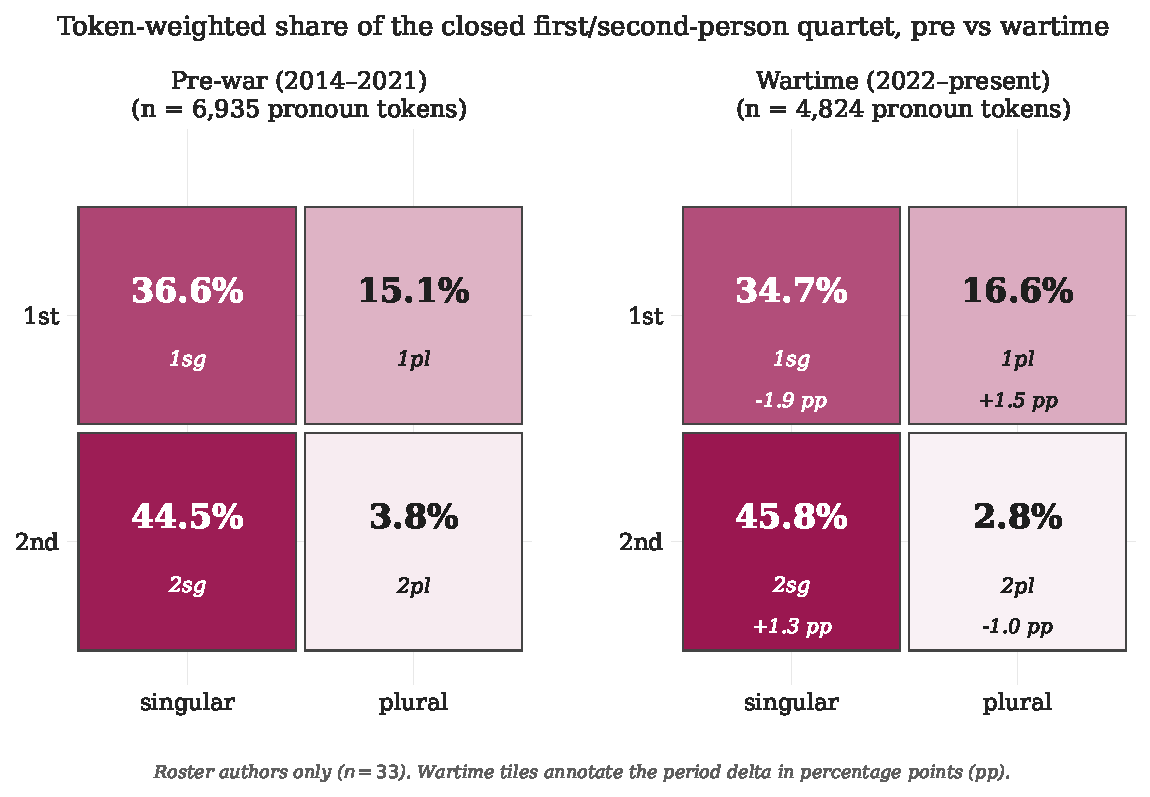
\includegraphics[width=0.85\textwidth]{fig_narr_7_person_number_redistribution.pdf}
\caption{Pre-war (left) vs.\ wartime (right) token-weighted share matrices for the closed first/second-person quartet \{1sg, 1pl, 2sg, 2pl\}, roster authors only. Wartime tiles annotate the period delta in percentage points. The plural column reweights toward 1st-person between the two panels; the within-plural conditional 1pl share and the cross-product odds ratio are reported in the body text above.}
\label{fig:rq1-pnum}
\end{figure}

\subsubsection{Temporal trajectory and breakpoint detection}

The corresponding per-pronoun temporal trajectories under the adaptive 35-bin partition described in Methods (\S\ref{sec:methods})---with the piecewise weighted-least-squares fit and the unsupervised PELT change-point series overlaid---are reported in Appendix~\ref{app:breakpoint} (Figure~\ref{fig:rq1-breakpoint}). The 1pl trajectory exhibits a level shift at the 2022 knot with $\hat{\beta}_{2022} = +0.20$ ($p = 0.051$, marginal), corresponding to the rise that the specification curve and the heterogeneous individual trajectories in RQ2 (below) recover. The unsupervised PELT pass on the 1pl series independently identifies two change-points within four months of one another (2022-03-01 and 2023-02-10), bracketing the post-invasion window. Other cells return either an earlier (2014) shift (1sg: $\hat{\beta}_{2014} = +0.10$, $p = 0.0003$, corresponding to the Donbas-onset) or no detectable break (2sg, 3pl). Taken together, the breakpoint regression and PELT detection identify 2022 as the most plausible single change-point for the 1pl series.

Figure~\ref{fig:rq1-timeseries} replots the 1pl share at annual resolution within the closed quartet, stratified by language. The Ukrainian-language series is dense enough across the entire window (large solid dots) to support visual inference: the bootstrap-95\,\% ribbon widens after 2022 because the per-year poem count thins, but the central tendency is uniformly above the pre-2014 baseline and remains there through 2025. The Russian-language series is supported by $\geq 10$ poems per year only through 2022 (faded dots after); the post-2022 Russian-stratum trajectory should therefore be read against the small-$n$ caveat embedded in the figure rather than against the central-tendency line.

\begin{figure}[h]
\centering
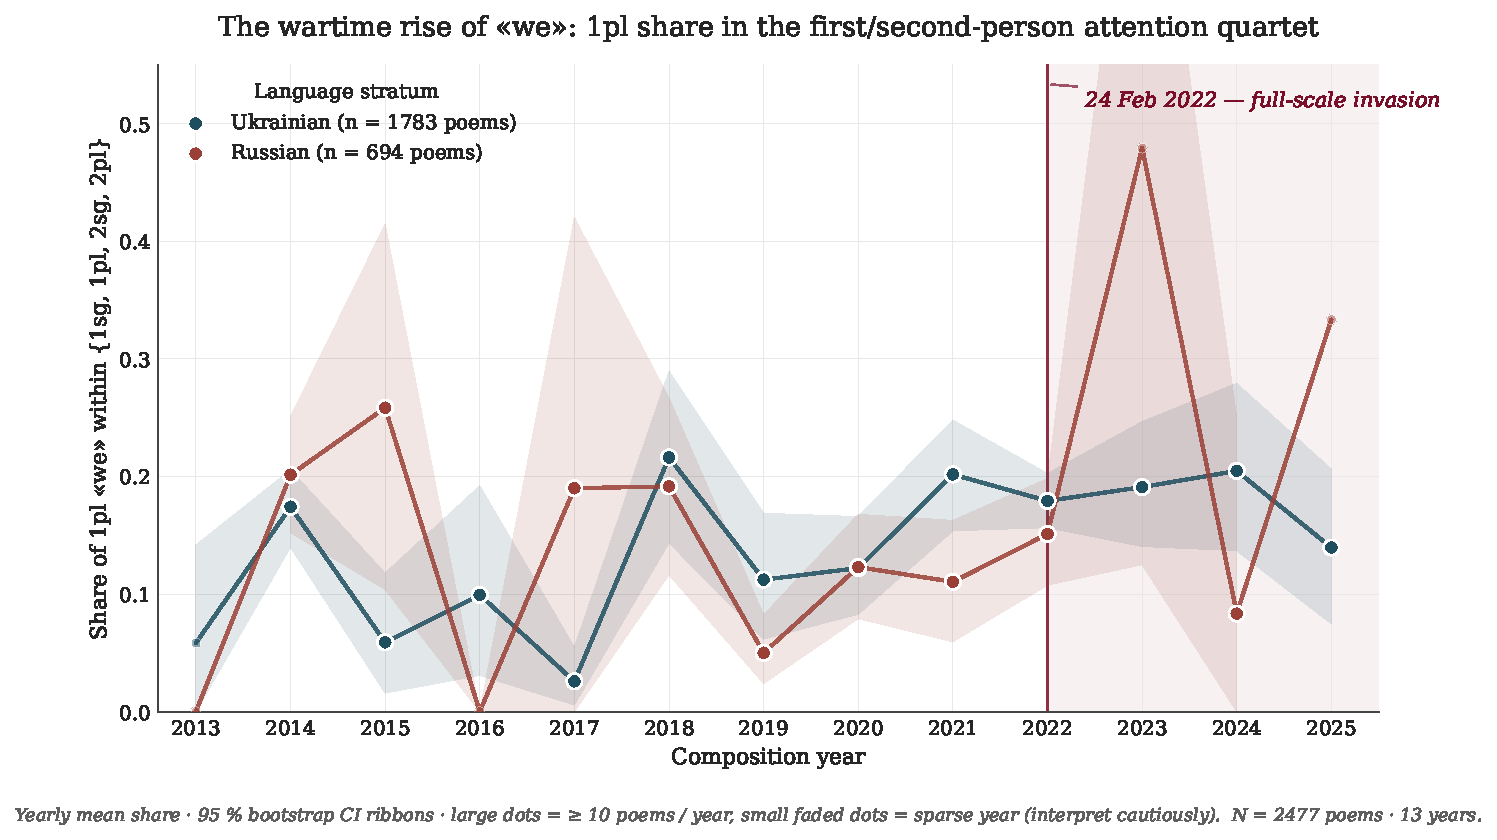
\includegraphics[width=0.95\textwidth]{fig_narr_1_time_series_we_rises.pdf}
\caption{Annual mean 1pl share within the closed first/second-person quartet, 2013--2025, by language stratum. Large solid markers denote years with $\geq 10$ poems in the stratum; small faded markers denote sparse years (interpret cautiously). Shaded ribbons are bootstrap 95\,\% CI around the per-year mean. The vertical wine bar marks 24 February 2022.}
\label{fig:rq1-timeseries}
\end{figure}

Across both language strata and under both the Poisson and the negative-binomial specifications, no within-author cell-level rate shift across the 24 February 2022 cutpoint survives the BH-FDR confirmatory criterion at $\alpha = 0.05$. The 1pl point estimates are uniformly positive (Ukrainian: IRR $= 1.20$; Russian: IRR $= 1.08$; pooled: IRR $= 1.18$) and the 2pl estimates are uniformly negative, but the corpus-clustered standard errors and the wild-cluster bootstrap render every cell-level claim non-significant after multiplicity correction. The corpus-level mean therefore cannot be read as having undergone a homogeneous, statistically detectable post-invasion shift in any single pronoun cell; whether that null reflects the absence of an effect or the presence of countervailing author-level trajectories is the question that the next section addresses directly.

\subsection{Individual Author Trajectories and Heterogeneity }
\label{sec:results-rq2}

For each of the four pronoun cells \{1sg, 1pl, 2sg, 2pl\} and each language stratum, we fit a poem-level negative-binomial hierarchical model with an author-level random slope on the period indicator, four chains of 2{,}000 draws after a 2{,}000-iteration warm-up via NUTS in Bambi (PyMC backend), $\widehat{R} < 1.02$ across all monitored parameters. Inference is summarized by 95\,\% highest-density intervals (HDIs) and by the posterior probability of direction $\Pr(\delta > 0\,|\,\text{data})$, with BH-style $q$-direction control applied within each cell.

\subsubsection{Population-level period shift after partial pooling}

The hierarchical population-level shifts replicate the RQ1 null (Table~\ref{tab:rq2-pop}). All twelve cell-by-stratum HDIs include zero; the smallest $q_{\text{direction}}$ in the pooled stratum is $0.41$ (1sg and 1pl), and the smallest in any stratum is $0.24$ (Russian 2sg). The hierarchical posteriors do, however, sharpen the directional reading of the RQ1 specification curve: the pooled-stratum 1pl population shift posterior places $76\,\%$ of mass above zero (posterior mean rate ratio $= 1.14$, $95\,\%$ HDI $= [0.77, 1.65]$), and the pooled 2pl shift sits at posterior mean rate ratio $1.06$ with HDI $[0.54, 2.01]$.

\begin{table}[h]
\caption{Population-level period shift (posterior summaries from the hierarchical NB random-slope model). All twelve HDIs include zero; no cell carries $q_{\text{direction}} < 0.05$.}
\label{tab:rq2-pop}
\centering
\small
\begin{tabular}{llrrrr}
\toprule
Stratum & Cell & RR (post.\ mean) & HDI95 & $\Pr(\delta > 0)$ & $q_{\text{direction}}$ \\
\midrule
Pooled & 1sg & 0.88 & [0.64, 1.20] & 0.22 & 0.41 \\
Pooled & 1pl & 1.14 & [0.77, 1.65] & 0.76 & 0.41 \\
Pooled & 2sg & 0.90 & [0.66, 1.21] & 0.24 & 0.41 \\
Pooled & 2pl (\textukrainian{ви}) & 1.06 & [0.54, 2.01] & 0.59 & 0.41 \\
Ukrainian & 1sg & 0.96 & [0.70, 1.31] & 0.41 & 0.50 \\
Ukrainian & 1pl & 1.19 & [0.80, 1.74] & 0.81 & 0.48 \\
Ukrainian & 2sg & 0.84 & [0.62, 1.13] & 0.13 & 0.48 \\
Ukrainian & 2pl (\textukrainian{ви}) & 0.94 & [0.43, 1.95] & 0.45 & 0.50 \\
Russian & 1sg & 0.78 & [0.25, 1.92] & 0.29 & 0.29 \\
Russian & 1pl & 1.41 & [0.55, 3.18] & 0.80 & 0.26 \\
Russian & 2sg & 1.57 & [0.86, 2.73] & 0.94 & 0.24 \\
Russian & 2pl (\textukrainian{ви}) & 1.73 & [0.44, 6.79] & 0.79 & 0.26 \\
\bottomrule
\end{tabular}
\end{table}

\subsubsection{Author random-slope variance}

We find that the aggregate null masks substantial author-level heterogeneity. In the pooled stratum, the posterior standard deviation of the author-level period-shift deviation (i.e.\ each author's offset from the population mean on the log-rate scale) is $\sigma_{\delta} = 0.50$ for 1sg, $0.56$ for 1pl, and $0.53$ for 2sg, magnitudes comparable to the population mean itself. On the rate-ratio scale, individual authors range from $\mathrm{RR} = 0.42$ to $\mathrm{RR} = 4.70$ on the 1pl cell, with the highest five posterior means clustered around authors who took on documented frontline or combat-medic roles after February 2022 (Mitrov $4.70$, Kiva $2.97$, Chornohuz $2.78$, Zharikova $2.57$, Khersonsky $2.00$; all five carry $\Pr(\delta > 0\,|\,\text{data}) > 0.96$) and the lowest three clustered around older Kyiv-resident poets who curtailed posting or evacuated in 2022 (Babkina $0.42$, Andrusiak $0.43$, Falkovych $0.43$; all three carry $\Pr(\delta > 0\,|\,\text{data}) < 0.11$). Two authors in the pooled stratum have a 1pl deviation HDI that excludes zero in the positive direction and one has $q_{\text{direction}} < 0.05$; none has a negative-direction HDI excluding zero.

The 2sg cell is the only one in which posterior heterogeneity runs in both directions: three authors carry positive 2sg deviation HDIs excluding zero and three carry negative ones, with two passing $q_{\text{direction}} < 0.05$. The 1sg cell is dominantly negative on the population mean (RR $= 0.88$) but its author-level posteriors include two strongly positive outliers (HDI excluding zero, $q_{\text{direction}} < 0.05$ for one), consistent with a small subset of poets shifting more weight onto the lyric ``I'' even as the corpus mean drifts the other way.

Figure~\ref{fig:rq2-trajectories} (Appendix~\ref{app:trajectories}) displays each roster author's pre-2022 position in the (1sg-share, 1pl-share) plane of the closed quartet together with an arrow to their wartime position. Pale-cream arrows show the full roster; eight narratively notable authors are highlighted by documented wartime situation---crimson for mobilized poets in frontline or civic-military positions (Mitrov, Chornohuz, Kiva, Zhadan), deep teal for residentially stable poets who remained in place through the cutpoint (Kruk, Zharikova), and muted bronze for poets displaced through the cutpoint, in-country or abroad (Falkovych, evacuated within Ukraine; Khersonsky, who fled Odesa for Italy)---with leader-line labels. The colour encodes biographical situation, not outcome: the arrow geometry carries the direction of each poet's drift, so that the displaced bucket can hold both Falkovych, whose 1pl recedes, and Khersonsky, whose 1pl rises. The cloud of arrows visibly disperses rather than coheres: a small high-mobility cluster (Mitrov, Kiva, Chornohuz, Zharikova) translates simultaneously up in the 1pl axis and left in the 1sg axis, while a separate cluster (Falkovych, Babkina, Andrusiak) drifts in the opposite direction. The displacement structure is the geometric counterpart of the random-slope variance reported in the preceding paragraph.

\subsubsection{Caterpillar of the 1pl per-author posterior}

Figure~\ref{fig:rq2-caterpillar} displays the per-author posterior total period-shift on the 1pl cell in the pooled stratum, the cell that hosts the strongest cross-author dispersion identified in \S~\ref{sec:results-rq2}. Authors are sorted by posterior mean total shift (most positive at top, most negative at bottom); the top-five and bottom-five authors are colored in the literary palette and labelled with their posterior-mean rate ratio, while the middle band of $23$ authors is greyed as context. The figure is restricted to the 1pl cell deliberately, both to fit a single printed page with named author labels and to focus the visual on the cell that carries the manuscript's heterogeneity finding. The three remaining cells display qualitatively similar dispersion patterns; their analogous caterpillars are produced by the modeling script and are reported in the supplementary material.

\begin{figure}[h]
\centering
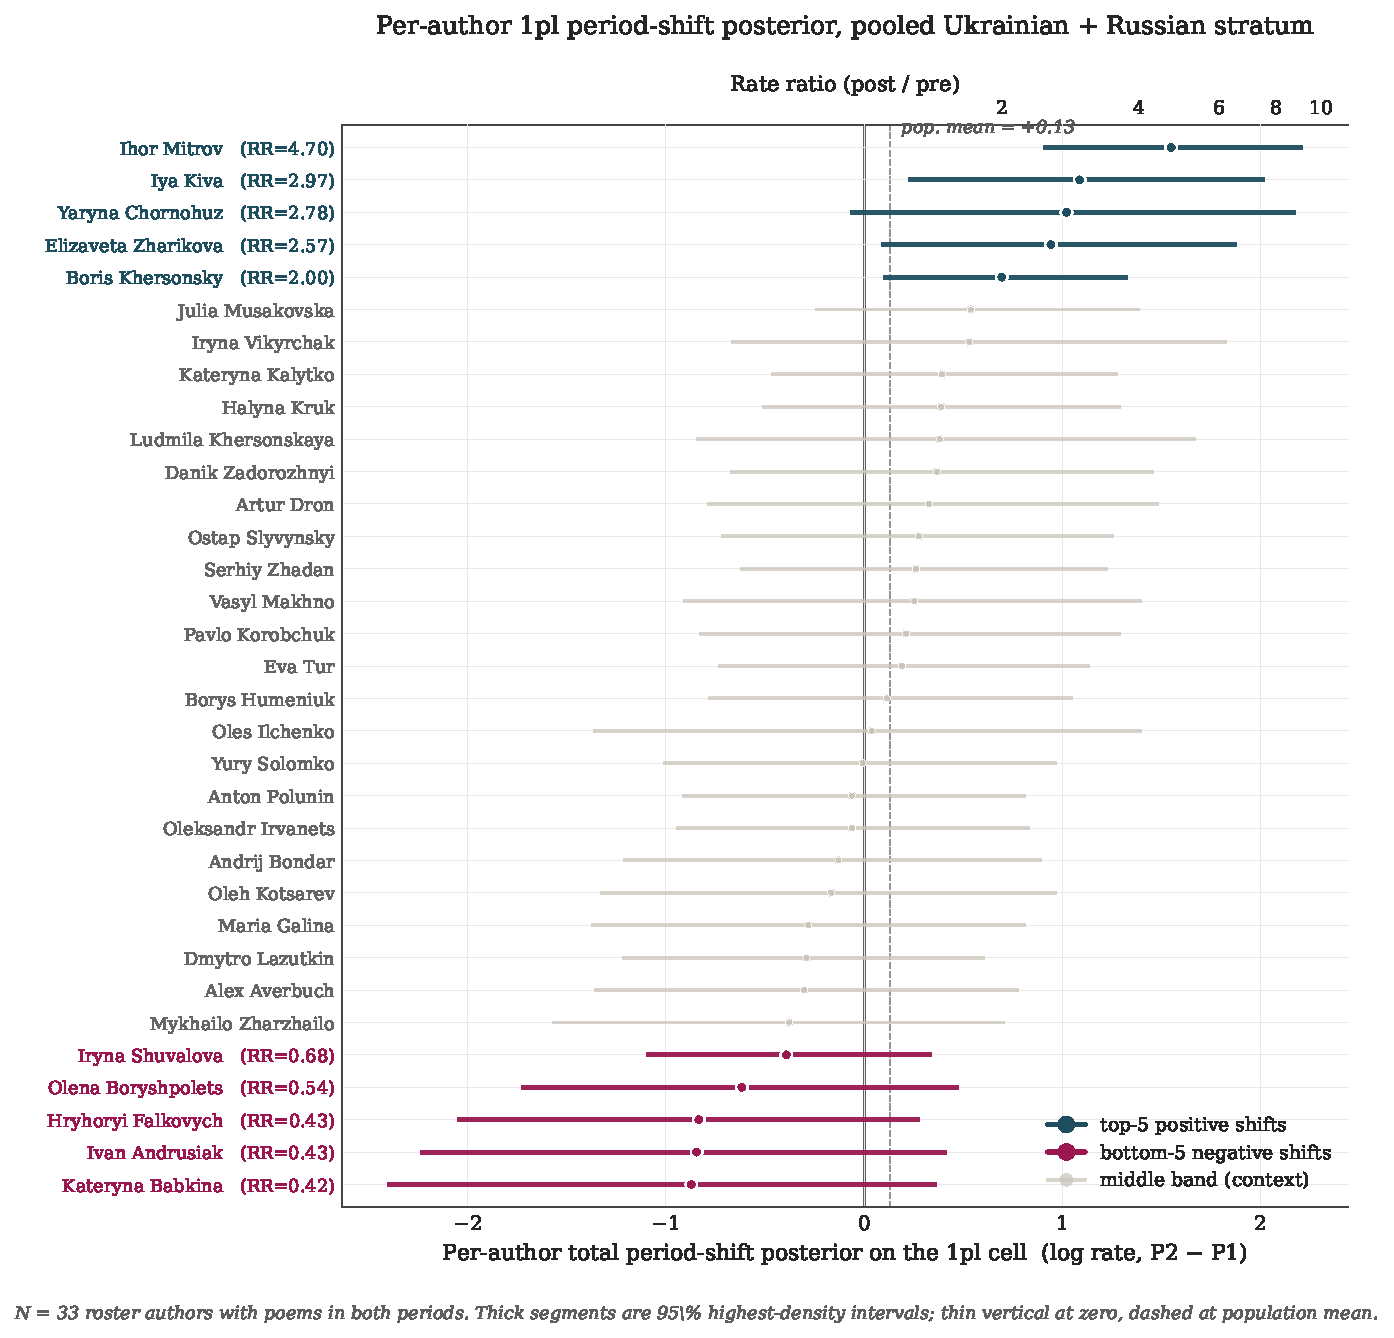
\includegraphics[width=0.92\textwidth]{fig_narr_8_caterpillar_1pl_focused.pdf}
\caption{Per-author posterior total period-shift on the 1pl cell, pooled Ukrainian + Russian stratum. Each row is one author; thick segments are 95\,\% highest-density intervals; the thin vertical at zero marks the no-shift null; the dashed vertical marks the across-author population mean. Top-five authors (deep-teal) and bottom-five authors (burgundy) are labeled with their posterior-mean rate ratio; the middle band of $23$ authors is greyed for context. The secondary upper axis re-expresses the log-rate shift on the multiplicative rate-ratio scale.}
\label{fig:rq2-caterpillar}
\end{figure}

\subsubsection{RQ2 summary}

The aggregate corpus-level null established by RQ1 conceals a heterogeneous, biographically-conditioned distribution of author-level trajectories. The 1pl cell hosts a cluster of strongly positive shifts among poets with documented post-2022 civic or military roles and a parallel cluster of negative shifts among older Kyiv-resident poets and post-2022 evacuees, while the 2sg cell is uniquely bidirectional. The population-level posteriors return the same null pattern as the frequentist GLMs (Table~\ref{tab:rq2-pop}), but the author-level posteriors document substantial cross-author variance that the corpus mean integrates out.

Figure~\ref{fig:rq2-cases} unpacks the author-level finding for six poets selected to span the heterogeneity reported above. Each panel plots the named poet's per-year 1pl share in the closed quartet with the 24 February 2022 cutpoint marked. The three frontline/combat-medic poets in the top row (Mitrov, Kiva, Chornohuz) and Serhiy Zhadan in the lower-left panel exhibit visible step-ups across the cutpoint; Boris Khersonsky shows a delayed wartime spike concentrated in 2023; Hryhoryi Falkovych's per-year 1pl rate falls and his archive entries thin after 2022, consistent with the negative posterior tail. The six per-year trajectories anchor the population posteriors (Table~\ref{tab:rq2-pop}) and the random-slope deviation summaries (\S~\ref{sec:results-rq2}) to specific, traceable individual records.

\begin{figure}[h]
\centering
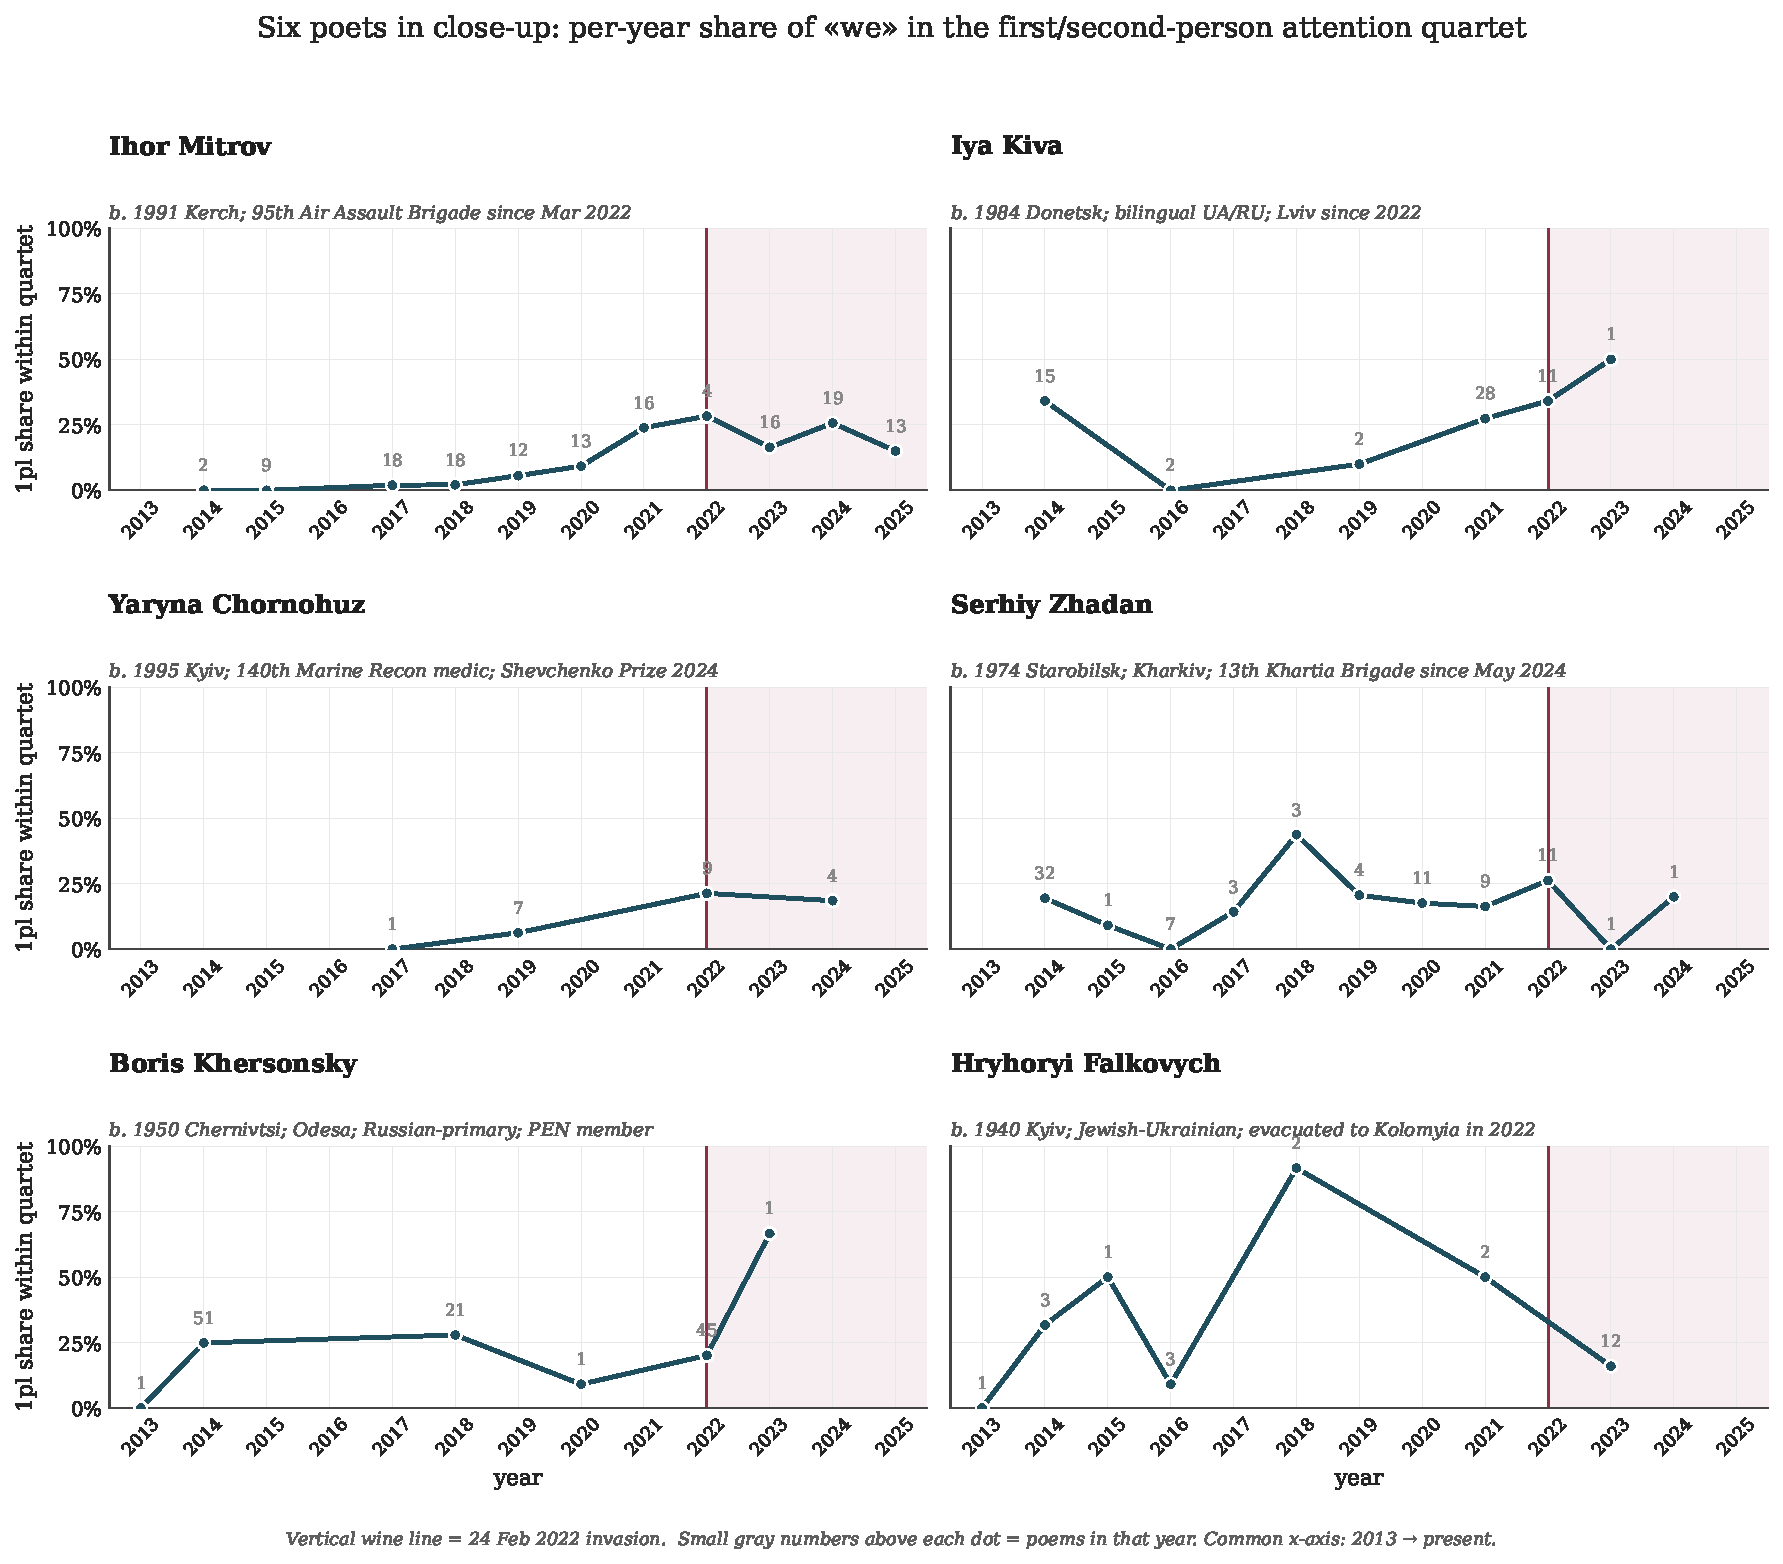
\includegraphics[width=0.98\textwidth]{fig_narr_5_case_study_poets.pdf}
\caption{Per-year 1pl share within the closed first/second-person quartet for six poets selected from the random-slope posteriors. Each panel is one poet; vertical wine bar marks 24 February 2022; small grey numbers above each dot are the poem count in that year. Biographic taglines beneath each title summarize the wartime context that the panel records.}
\label{fig:rq2-cases}
\end{figure}

\subsection{Lexical-Syntactic Anchoring of the Wartime First Person}
\label{sec:results-rq3}

The corpus-level null and the author-level dispersion together establish that the wartime cutpoint does not produce a single homogeneous frequency shift on any pronoun cell. They leave open a second-order question that the rate models cannot address: among the pronouns that do appear, has the lexical-syntactic company each cell keeps shifted across the cutpoint? The dependency-parsed collocation layer (\S\ref{sec:methods-collocations}) answers that question by recovering, for every personal-pronoun token in the corpus, the head lemma it governs in the universal-dependency parse, and testing which head lemmas shift their association with the pronoun between 2014--2021 and post-2022.

\subsubsection{Survivors of multiplicity control}

Across the eight (language, cell) families and a combined inventory of 262 candidate head lemmas with at least five corpus-wide co-occurrences, eleven head-lemma collocates survive the Benjamini--Hochberg correction at $q < 0.10$. Table~\ref{tab:rq3-bh-survivors} reports the full list. The Ukrainian-stratum survivors concentrate on the 1pl, 2sg, and 1sg cells; the Russian-stratum survivors concentrate almost entirely on the 1sg cell. The 2pl cells in both strata host no survivors, consistent with their thin token counts and the corresponding scarcity of repeatable head-lemma collocations to test against the noise floor.

\begin{table}[h]
\centering
\caption{Head-lemma collocates of personal pronouns surviving Benjamini--Hochberg multiplicity control at $q < 0.10$ within each (language, cell) family. ``Pre'' and ``Post'' are raw counts of stanza-level pronoun-governs-head co-occurrences from the Stanza dependency parse. $G^2$ is the log-likelihood ratio statistic on the period $\times$ with-this-head $2\times 2$ table. A $q$-value of $0.000$ denotes $q < 10^{-5}$.}
\label{tab:rq3-bh-survivors}
\small
\begin{tabular}{llllrrrr}
\toprule
Lang. & Cell & Deprel & Head lemma & Pre & Post & $G^2$ & $q_{\text{BH}}$ \\
\midrule
Ukrainian & 1pl & nsubj & \textukrainian{мусити} (must)        &  0 & 13 & 20.3 & 0.007 \\
Ukrainian & 2sg & nsubj & \textukrainian{хотіти} (want)        &  7 & 28 & 19.3 & 0.013 \\
Ukrainian & 1sg & nsubj & \textukrainian{стати} (become)       &  3 & 18 & 16.4 & 0.069 \\
Ukrainian & 1sg & nsubj & \textukrainian{говорити} (speak)     & 26 &  3 & 15.4 & 0.069 \\
Russian   & 1sg & nsubj & \textukrainian{называть} (name/call) &  0 & 30 & 79.5 & 0.000 \\
Russian   & 1sg & nsubj & \textukrainian{благодарный} (grateful) &  0 & 13 & 34.0 & 0.000 \\
Russian   & 1sg & nsubj & \textukrainian{казаться} (seem)      &  0 & 11 & 28.7 & 0.000 \\
Russian   & 1sg & iobj  & \textukrainian{казаться} (seems-to-me) &  5 & 14 & 17.8 & 0.005 \\
Russian   & 1sg & iobj  & \textukrainian{написать} (write-to-me) &  0 &  5 & 13.0 & 0.041 \\
Russian   & 1sg & nsubj & \textukrainian{делать} (do)          &  0 &  5 & 13.0 & 0.041 \\
Russian   & 1sg & nsubj & \textukrainian{любить} (love)        & 27 &  1 & 11.4 & 0.082 \\
\bottomrule
\end{tabular}
\end{table}

\subsubsection{Ukrainian 1pl: the emergence of a deontic ``we must''}

The single survivor on the Ukrainian 1pl cell is the modal verb \textukrainian{мусити} (must / have to) as the dependency head of a 1pl subject. The verb is absent from the pre-2022 corpus as a 1pl-nsubj governor and accumulates thirteen post-2022 occurrences, at $q = 0.007$ and $G^2 = 20.3$. This is the only head-lemma collocate that survives multiplicity control on the 1pl cell in either language stratum, and it does so cleanly: the pre-2022 zero count is exhaustive across the roster, so the post-2022 occurrences are not a redistribution of an existing pattern but the genuine appearance of a construction that the corpus did not previously sustain.

The substantive reading is that the wartime Ukrainian 1pl carries a deontic load it did not carry before. The pre-war collective ``we'' was descriptive or existential; the wartime collective ``we'' is exhorted into duty. This delivers, at the dependency-parse level, the kind of legitimization-strategy encoding that \citet{reyes2011strategies} identifies as wartime-discourse signature: obligation is grafted directly onto the in-group pronoun rather than expressed through separate sentential frames.

A second pattern accompanies this single survivor at directional level (Figure~\ref{fig:rq3-barbell-ukr-1pl}). The pre-2022 1pl preferred head lemmas of habitual or mundane action (\textukrainian{могти} ``be able'', \textukrainian{носити} ``carry'', \textukrainian{прокинутися} ``wake'', \textukrainian{ховатися} ``hide'', \textukrainian{брати} ``take''). The post-2022 1pl preferred head lemmas of communication, cognition, and perception (\textukrainian{говорити} ``speak'', \textukrainian{ставати} ``become'', \textukrainian{думати} ``think'', \textukrainian{вийти} ``come out'', \textukrainian{бачити} ``see'', \textukrainian{дивитися} ``look''). None of these individual movements survives BH correction, but the directional consistency across nearly thirty head lemmas indicates that the deontic survivor sits in a broader semantic relocation: the wartime ``we'' becomes a speaking, thinking, and witnessing subject rather than an acting and concealing one.

\begin{figure}[h]
\centering
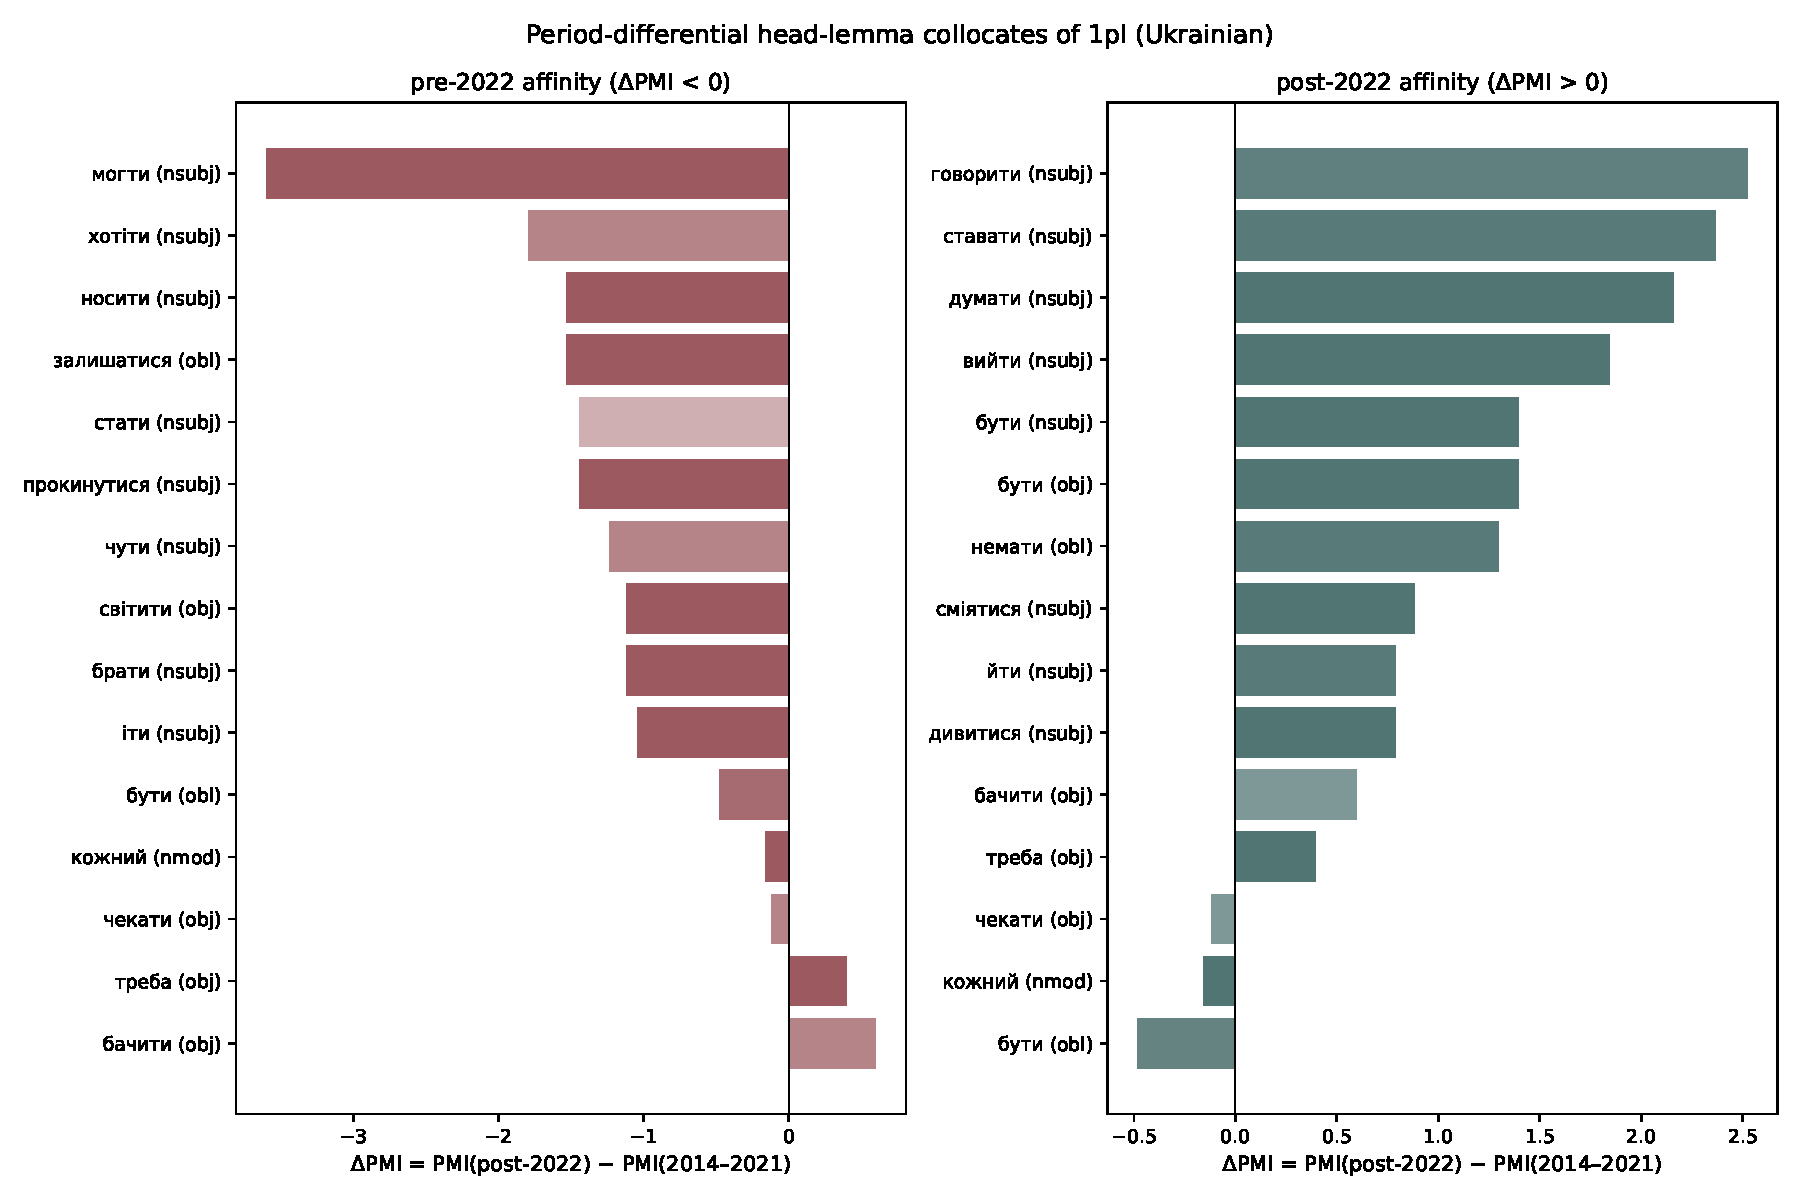
\includegraphics[width=0.95\textwidth]{fig_narr_9_barbell_ukr_1pl.pdf}
\caption{Period-differential head-lemma collocates of the Ukrainian 1pl cell, ranked by $\Delta\mathrm{PMI}$. Left panel: pre-2022 affinity (top fifteen head lemmas with $\Delta\mathrm{PMI} < 0$, i.e.\ preferred by 1pl in 2014--2021). Right panel: post-2022 affinity (top fifteen with $\Delta\mathrm{PMI} > 0$). Bar opacity is proportional to $1 - q_{\text{BH}}$, so confidently-shifted lemmas appear darker. Only \textukrainian{мусити} survives BH at $q < 0.05$; the figure documents the directional concentration in which that single survivor sits.}
\label{fig:rq3-barbell-ukr-1pl}
\end{figure}

\subsubsection{Ukrainian 2sg: the addressee as object of desire}

The Ukrainian 2sg cell's BH survivor is \textukrainian{хотіти} (want), which rises from seven pre-2022 occurrences as a 2sg-nsubj governor to twenty-eight post-2022, at $q = 0.013$ and $G^2 = 19.3$. Together with the directional rises in \textukrainian{знати} (know), \textukrainian{чекати} (wait), \textukrainian{любити} (love), \textukrainian{прийти} (come), and \textukrainian{бачити} (see), and the directional falls in \textukrainian{взяти} (take), \textukrainian{шукати} (seek), \textukrainian{написати} (write), \textukrainian{казати} (say), and \textukrainian{думати} (think), the 2sg drifts from a paradigm in which the intimate addressee thinks, writes, and seeks toward one in which the same addressee wants, knows, waits, and loves. Figure~\ref{fig:rq3-barbell-ukr-2sg} shows the full distribution. It indicates that one of the two directions in which the wartime 2sg moves is the intensification of an affective, elegiac, beloved-addressed register.

\begin{figure}[h]
\centering
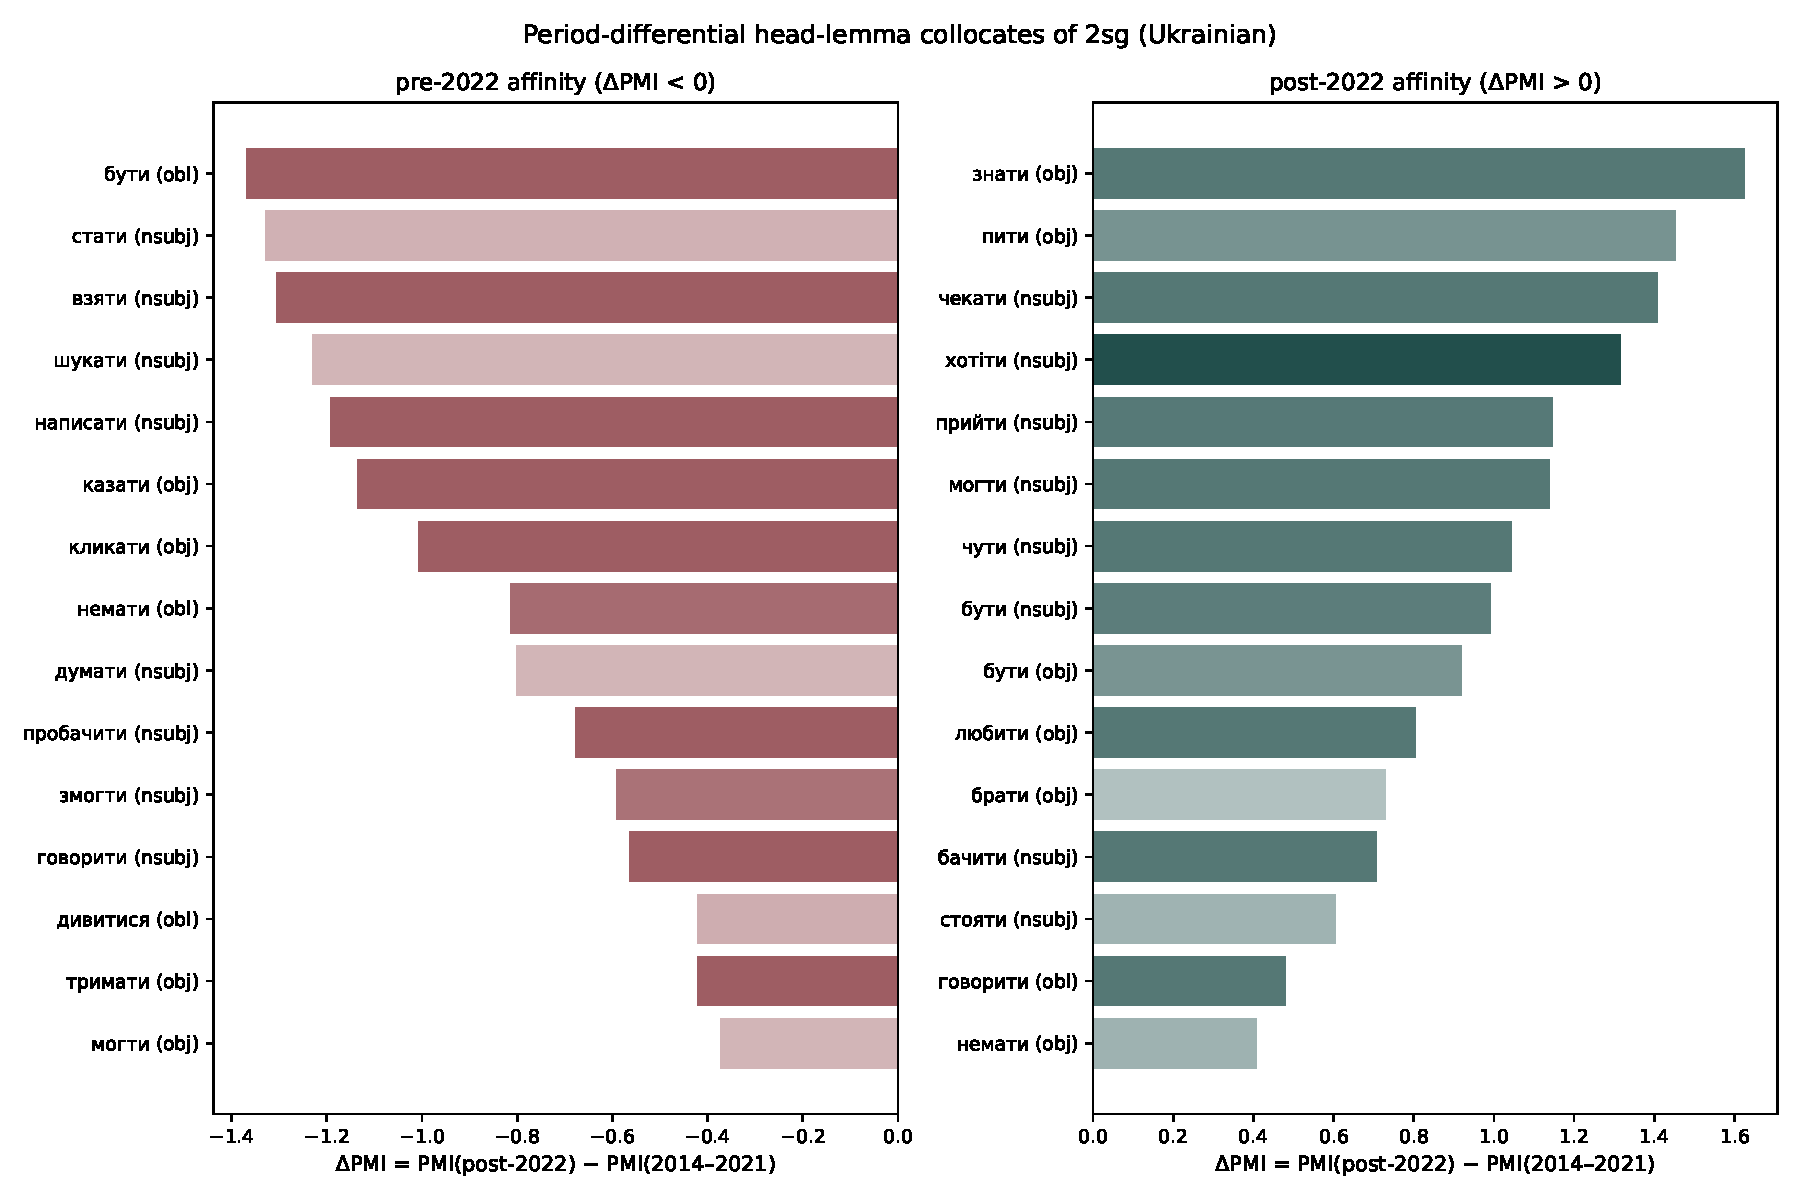
\includegraphics[width=0.95\textwidth]{fig_narr_10_barbell_ukr_2sg.pdf}
\caption{Period-differential head-lemma collocates of the Ukrainian 2sg cell. Conventions as in Figure~\ref{fig:rq3-barbell-ukr-1pl}. The BH survivor is \textukrainian{хотіти}; the directional companions in the right-panel cluster are predominantly affective and perceptual verbs.}
\label{fig:rq3-barbell-ukr-2sg}
\end{figure}

\subsubsection{Russian 1sg: the lyric subject reorganises}

The Russian 1sg cell is the only cell in either stratum where multiplicity control admits a dense cluster of survivors. Six head lemmas pass $q < 0.05$, with a seventh (\textukrainian{любить}) at $q = 0.082$. The dominant survivor is \textukrainian{называть} (to name / call), which rises from zero pre-2022 occurrences as a 1sg-nsubj governor to thirty post-2022 at $G^2 = 79.5$. Two further nsubj governors emerge from zero with comparably large statistics: \textukrainian{благодарный} (grateful, $0 \to 13$) and \textukrainian{казаться} (seem, $0 \to 11$). The same lemma \textukrainian{казаться} also rises as an indirect-object governor (5 $\to$ 14, $q = 0.005$), reflecting the syntactically distinct ``it seems to me'' construction. \textukrainian{Любить} (love) collapses in the opposite direction from twenty-seven pre-2022 occurrences to a single post-2022 occurrence.

The pattern is a verbal restructuring of the Russian-language lyric subject. The pre-war Russian ``I love'' essentially exits the corpus. The post-war Russian 1sg gains an attitudinal register (grateful, seeming) and a naming register (\textukrainian{называть}), which in the post-2022 Russophone poetic record is a verb often loaded with the work of confronting imperial cultural inheritance: naming places, victims, and perpetrators. Figure~\ref{fig:rq3-barbell-rus-1sg} displays the full distribution.

This Russian 1sg cluster must, however, be read with a strong caveat. The log-likelihood collocation test treats each pronoun--head co-occurrence as an independent draw, but lyric poems repeat the same construction anaphorically, and a token-level audit shows that the cell's headline survivors are not corpus-wide shifts but the signature of a single poet. All thirty post-2022 \textukrainian{называть} tokens, all thirteen \textukrainian{благодарный} tokens, and all eleven 1sg-nsubj \textukrainian{казаться} tokens originate in anaphoric list-poems by one author (Yury Solomko); the lone post-2022 \textukrainian{любить} token is also his. Because these counts violate the independence assumption through within-poem repetition (pseudo-replication), their extreme $q$-values overstate the evidence, and the apparent concentration of survivors on the Russian 1sg cell does not license the inference that the most dramatic restructuring of the lyric subject occurs in the Russian-language stratum. The distributionally robust collocation shifts in this corpus are instead the two Ukrainian survivors that spread across many poets: \textukrainian{хотіти} on the 2sg cell (28 post-2022 tokens across nineteen poems and ten authors) and, more modestly, \textukrainian{мусити} on the 1pl cell (thirteen tokens across six poems and five authors).

\begin{figure}[h]
\centering
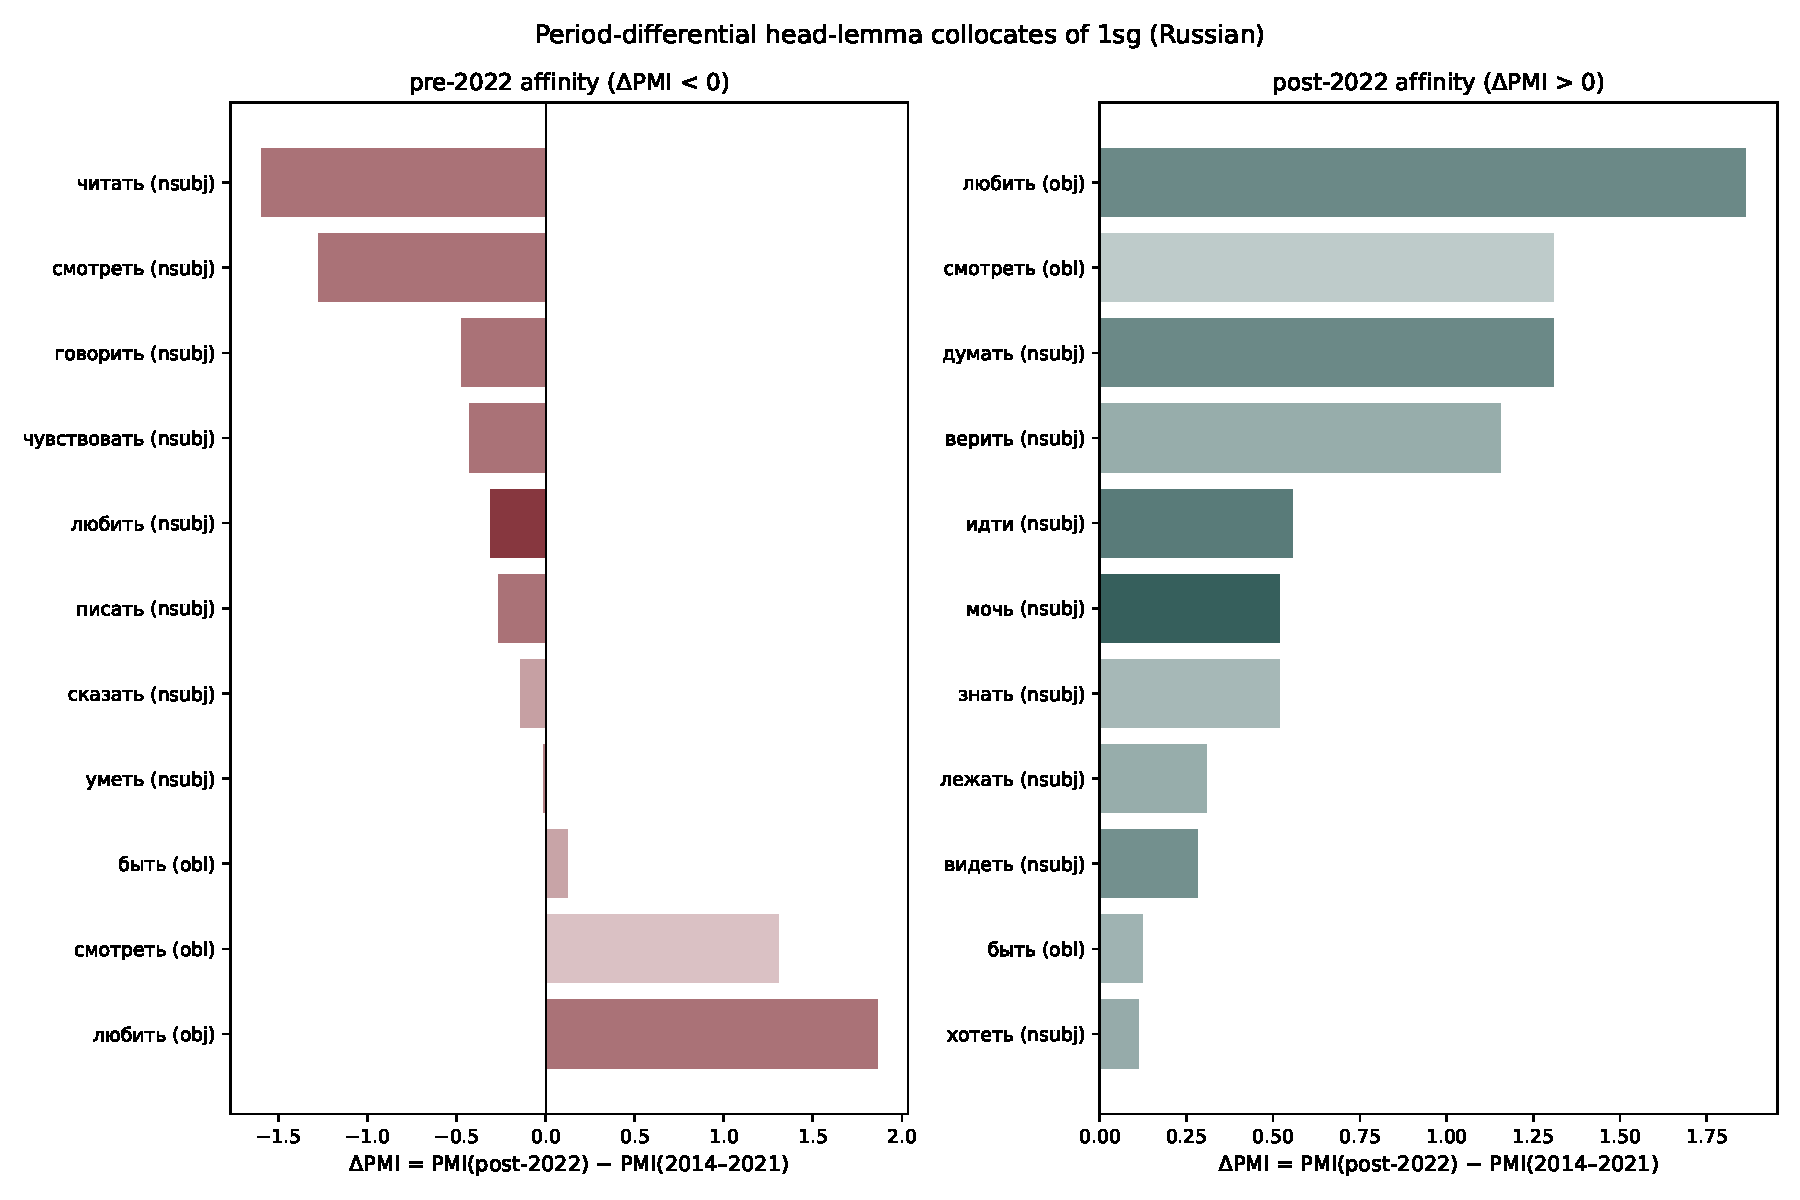
\includegraphics[width=0.95\textwidth]{fig_narr_11_barbell_rus_1sg.pdf}
\caption{Period-differential head-lemma collocates of the Russian 1sg cell. Conventions as in Figure~\ref{fig:rq3-barbell-ukr-1pl}. Six BH survivors at $q < 0.05$, with darker bars in the right panel; \textukrainian{любить} survives only marginally and appears in the left panel.}
\label{fig:rq3-barbell-rus-1sg}
\end{figure}

\subsubsection{Author-cluster decomposition: who speaks the deontic ``we''?}

The corpus-level survivor \textukrainian{мусити} is identified on the pooled stratum and is silent about which authors carry it. To answer that, we re-aggregate the dependency-parsed 1pl tokens by the RQ2 author clusters (\S\ref{sec:methods-collocations}). Table~\ref{tab:rq3-cluster-1pl} summarises the top emergent post-2022 1pl head lemmas within each cluster.

\begin{table}[h]
\centering
\caption{Top emergent post-2022 1pl head-lemma collocates within each author cluster, ranked by post-2022 raw count among lemmas with zero pre-2022 occurrences in that cluster. The retreat cluster contributes only ten post-2022 1pl tokens, too few to support any individual collocate claim, and is reported as a denominator note rather than a content row.}
\label{tab:rq3-cluster-1pl}
\small
\begin{tabular}{lll}
\toprule
Cluster (post-2022 1pl tokens) & Top emergent head lemmas (raw post-2022 count) & Register \\
\midrule
Mobilized (198) & \textukrainian{боятися} (fear, 4); \textukrainian{лишитися} (remain, 3); & existential, \\
                & \textukrainian{строить} (build, 3); \textukrainian{писати} (write, 2). & embodied \\
\addlinespace
Other (751)     & \textukrainian{мусити} (must, 13); \textukrainian{ми} as conjunct (6); & deontic, \\
                & \textukrainian{воювати} (wage war, 3); \textukrainian{битися} (fight, 3); & mobilizational \\
                & \textukrainian{сміятися} (laugh, 3); \textukrainian{спілкуватися} (communicate, 3). & \\
\addlinespace
Retreat (10)    & Sample too thin for cluster-conditional inference. & n/a \\
\bottomrule
\end{tabular}
\end{table}

The corpus-level survivor \textukrainian{мусити} is concentrated entirely in the ``other'' cluster, the non-frontline portion of the roster. The frontline-mobilized cluster, whose members carry documented civic-military roles, does not deploy \textukrainian{мусити} as a 1pl governor at all in the post-2022 sample. Its top emergent 1pl head lemmas are instead \textukrainian{боятися} (fear) and \textukrainian{лишитися} (remain). While the non-frontline roster performs the corpus-wide deontic and combative ``we'' that the population-level analysis recovers, the frontline poets articulate a different 1pl: one whose governing verbs are existential rather than exhortational, anchored in the lived stance of staying and being afraid rather than in the rhetorical stance of mobilization.

This decomposition supplies the empirical extension that the rate-level RQ2 analysis cannot deliver. The wartime ``we'' at the corpus level is a composite of two registers held by two different sub-populations of poets. The mobilizational register operates from outside the immediate physical war and frames it; the existential register operates from inside the war and inhabits it. The 1pl cell is one grammatical object, but the dependency-parse evidence localises at least two referentially distinct discursive objects beneath that single pronoun.

The collocation layer recovers a small but interpretable set of BH-controlled survivors that the rate-level analyses do not surface. The wartime Ukrainian 1pl gains a deontic head verb (\textukrainian{мусити}) that the pre-war corpus did not host. The wartime Ukrainian 2sg gains an affective head verb (\textukrainian{хотіти}) sitting in a broader move toward addressee-as-beloved. The wartime Russian 1sg undergoes the most dramatic verbal restructuring in the corpus, replacing \textukrainian{любить} with a naming and attitudinal register dominated by \textukrainian{называть}. The 2pl cells in both strata host no survivors, consistent with their thinner token counts. At the author-cluster level the corpus-level deontic ``we'' resolves into a referentially split phenomenon: the mobilizational verbs concentrate in the non-frontline roster, while the frontline-mobilized roster's wartime 1pl articulates an existential, embodied stance.

\section{Discussions}

\subsection{Synthesis: heterogeneous reaction, not homogeneous crystallization}
\label{sec:discussion-synthesis}

In conclusion, the 24 February 2022 cutpoint does not produce a homogeneous corpus-level linguistic shift in any individual person--number cell: under the confirmatory criterion of agreement between Poisson and negative-binomial GLMs plus wild-cluster bootstrap survival of BH-FDR control, no cell in either the Ukrainian or the Russian language stratum reaches significance, and the hierarchical Bayesian replication returns a parallel null at the population level (Table~\ref{tab:rq2-pop}). The same data, partitioned at the author level, document substantial heterogeneous variance: random-slope standard deviations on the open cells range from $0.50$ to $0.56$ log-units, with individual author period-shifts spanning approximately three log-units on the 1pl cell alone, and with both ends of the 2sg distribution populated by HDI-excludes-zero authors. The strongest positive 1pl shifts cluster among poets who took on documented civic-military roles after 2022 (Mitrov, Chornohuz, Zharikova, Kiva, Khersonsky), and the strongest negative 1pl shifts cluster among older Kyiv-resident poets and post-2022 evacuees (Babkina, Andrusiak, Falkovych). The invasion did not crystallize a single shared wartime ``we''; it polarized the deictic field along biographical lines that the corpus mean dissolves.

The collocation layer (\S\ref{sec:results-rq3}) refines this synthesis in two respects. First, although individual head-lemma collocates mostly fail to survive multiplicity control (consistent with the RQ1 corpus-level null at the rate level), the survivors that survive a distributional-robustness check are interpretively coherent: the wartime Ukrainian 1pl gains a deontic governor (\textukrainian{мусити}, ``must''), and the wartime Ukrainian 2sg gains an affective governor (\textukrainian{хотіти}, ``want''), each spread across many poets. The apparent Russian 1sg cluster (a naming and attitudinal register dominated by \textukrainian{называть}) is by contrast a pseudo-replication artifact concentrated in a single author and is set aside here (\S\ref{sec:results-rq3}). Where the rate-level analyses see a null, the collocation layer sees a small but coherent re-organisation of the verbal company the two robust Ukrainian pronoun cells keep. Second, the cluster decomposition of the Ukrainian 1pl collocates locates the corpus-level deontic survivor inside the non-frontline portion of the roster rather than the frontline-mobilized portion. While the non-frontline roster performs the corpus-wide mobilizational ``we'', the frontline poets articulate a 1pl whose governing verbs are existential rather than exhortational. The polarization that RQ2 identifies as biographical at the rate level extends, at the collocate level, to a clean register split: the same grammatical pronoun does at least two different kinds of discursive work in the same corpus.

\citet{billig1995banal}'s account of national flagging predicts that an existential rupture should increase the rate of banal, unreflective 1PL deixis among speakers who continue to operate within the imagined community. The RQ1 specification curve recovers exactly this directional signal (1pl is positive in $100\,\%$ of Ukrainian-stratum specifications and in the pooled stratum), but the magnitude does not survive BH-FDR correction. Read against the corpus mean, the wartime ``we'' is flagged but not statistically detectable as a corpus-level rate shift. Read at the author level, however, the strong positive 1pl posteriors concentrate not on the banal background of Ukrainian-language poetic discourse but on a specific subset of poets whose biographies underwent a categorical reclassification in 2022. This is precisely the reading licensed by \citet{brubaker2004ethnicity}'s reformulation of groupness as a contingent event: nationhood is not a property of the population but an achievement of categorization, mobilization, and discursive practice that some actors enact more intensively than others. \citet{brubaker2000beyond}'s decomposition of ``identity'' into identification, self-understanding, and commonality maps directly onto the RQ2 author panel: identification with the wartime collective is unevenly distributed even within a self-selected literary roster, and the 1pl rate is the trace that distribution leaves in the corpus.

The RQ3 collocation evidence adds a verbal-grammar register to the same callback. \citet{reyes2011strategies}'s legitimization-strategy framework, developed for post-2001 American political discourse, predicts that wartime in-group pronouns acquire obligation-bearing predicates as the speaker mobilises the audience into a duty-bound collective. The emergence of \textukrainian{мусити} as a 1pl-nsubj governor at $q = 0.007$, from a pre-war count of zero, is the dependency-parse footprint of that prediction in the Ukrainian poetic corpus. \citet{billig1995banal}'s ``banal'' 1pl is a flag that becomes more frequent; Reyes's deontic 1pl is a flag that, once raised, governs different verbs. The cluster decomposition shows further that this Reyesian deontic flag is carried by the non-frontline portion of the roster while the frontline poets articulate an existential rather than mobilizational 1pl, so the legitimization strategy and the lived-experience strategy occupy the same pronoun in different sub-populations of the corpus.

Figure~\ref{fig:disc-cohort} disaggregates the four-cell quartet by generation cohort to make the same point structurally. Across all five cohorts the four-cell composition is approximately stable for 1sg, 2sg, and 2pl (\textukrainian{ви}) from pre-2022 to wartime; the only cohort that registers a visibly larger 1pl share within the post-2022 panel is the $1990\text{s}$ cohort (the youngest fighting-age cohort in the roster), whose 1pl share more than doubles ($9\,\% \to 20\,\%$ within the closed quartet). The pre-1970 and 1970s cohorts show no comparable shift; the 1980s cohort moves very modestly. The cohort-conditional reading is consistent with \citet{onuch2022the}'s account of post-2022 civic Ukrainian identity as a generation-specific performative achievement: the wartime ``we'' that the corpus mean does not detect is concentrated in the cohort whose biographies were most directly reconfigured by the invasion.

\begin{figure}[h]
\centering
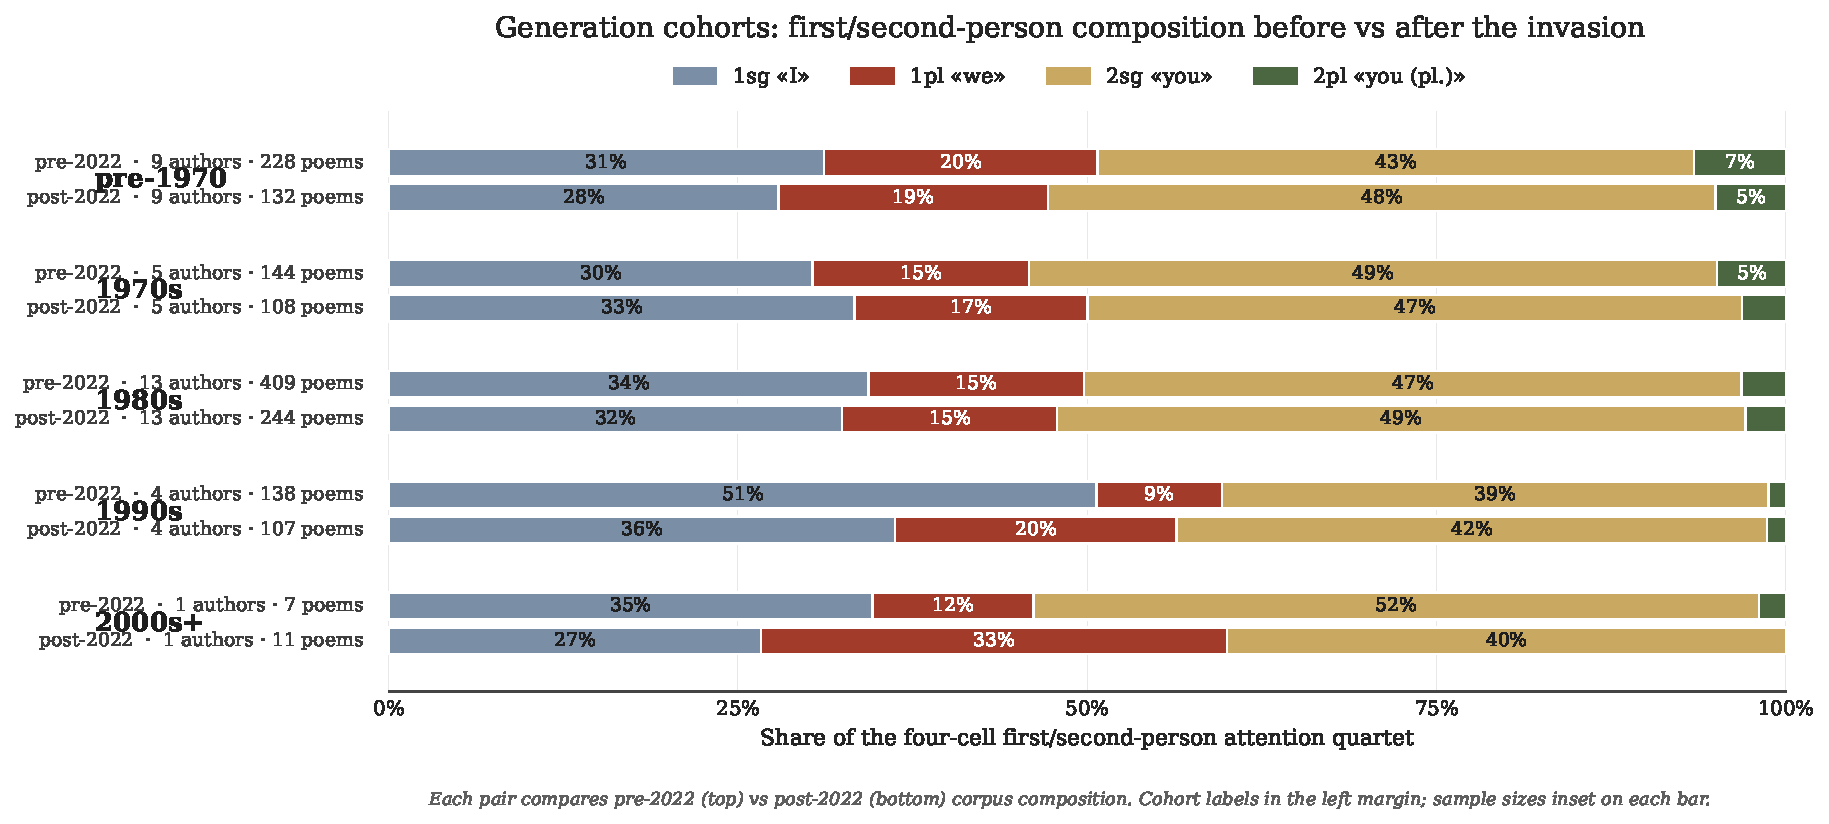
\includegraphics[width=0.98\textwidth]{fig_narr_4_generation_cohort_composition.pdf}
\caption{Cohort-by-period composition of the four-cell first/second-person attention quartet, roster authors only. Each pair compares pre-2022 (top bar) vs.\ post-2022 (bottom bar) corpus composition for one generation cohort. Cohort labels appear in the left margin; sample sizes (authors $\cdot$ poems) are inset on each bar. Cell colors: 1sg (slate), 1pl (rust), 2sg (gold), 2pl (forest). The 1990s cohort is the only one whose 1pl share more than doubles after the invasion.}
\label{fig:disc-cohort}
\end{figure}

\subsubsection{Sociolinguistic grounding: Kulyk, Onuch, and the post-2022 civic identity}

\citet{kulyk2022imperfect, kulyk2024language} documents a historically sharp post-2022 retreat of Russian from everyday Ukrainian language practice and a corresponding rise of civic Ukrainian identifications that crosscut ethnolinguistic categories. \citet{onuch2022the} frames the post-2022 civic Ukrainian nation as a generation-specific, performative achievement that crystallized through the experience of invasion. The author-level pattern reported in \S\ref{sec:results-rq2} aligns with both accounts in the specific direction they would predict: the positive 1pl cluster is dominated by poets whose post-2022 biographies record an explicitly performative civic-military realignment (Mitrov enlisted in the 95th Air Assault Brigade in March 2022; Chornohuz served continuously as a combat medic in the 140th Marine Reconnaissance Battalion and received the 2024 Shevchenko Prize for that work; Zharikova has served as a Territorial Defence combat medic since February 2022; Kiva is documented displacement from Donetsk to Lviv with a coincident shift toward Ukrainian-language composition; Khersonsky, a Russian-language poet long resident in Odesa, fled the city after February 2022 and has since been a fellow at the Civitella Ranieri Foundation in Italy, his post-2022 publishing shifting into a bilingual register). The negative 1pl cluster is dominated by older Kyiv-resident poets and post-2022 evacuees whose archive entries thin substantially after 2022 (Falkovych b.~1940, evacuated to Kolomyia; Andrusiak b.~1968; Babkina b.~1985 with documented Kyiv-Warsaw circulation post-2022). The corpus-level null and the structured author-level dispersion are therefore consistent: the post-2022 civic Ukrainian ``we'' is not a uniform banal flag in this poetic field, it is the differential mobilization of specific biographically situated speakers, and the corpus mean inevitably averages mobilization against retreat.

Figure~\ref{fig:disc-map} projects the same heterogeneity onto the authors' region of birth. The Kyiv-born sub-roster ($n = 5$) is the only in-country region whose mean wartime $\Delta$1pl-share is negative, consistent with the Falkovych / Babkina / Andrusiak cluster. The East-Ukraine and South-Ukraine sub-rosters carry the largest positive mean shifts (\,$+8.3\,$pp and $+9.6\,$pp respectively), reflecting authors with the most direct biographical exposure to the front line. The off-map ``born abroad'' panel ($n = 2$; Maria Galina, Arkadii Shtypel) is more positive still ($+12.1\,$pp), driven by relocated bilingual poets whose post-2022 publication shifted in the same direction as the East-Ukraine in-country pattern. The geographic structuring is consistent with the Kulyk/Onuch civic-identity framing: the wartime ``we'' is concentrated in those biographies for which the invasion was, in the most concrete sense, a re-categorization of their own ground.

\begin{figure}[h]
\centering
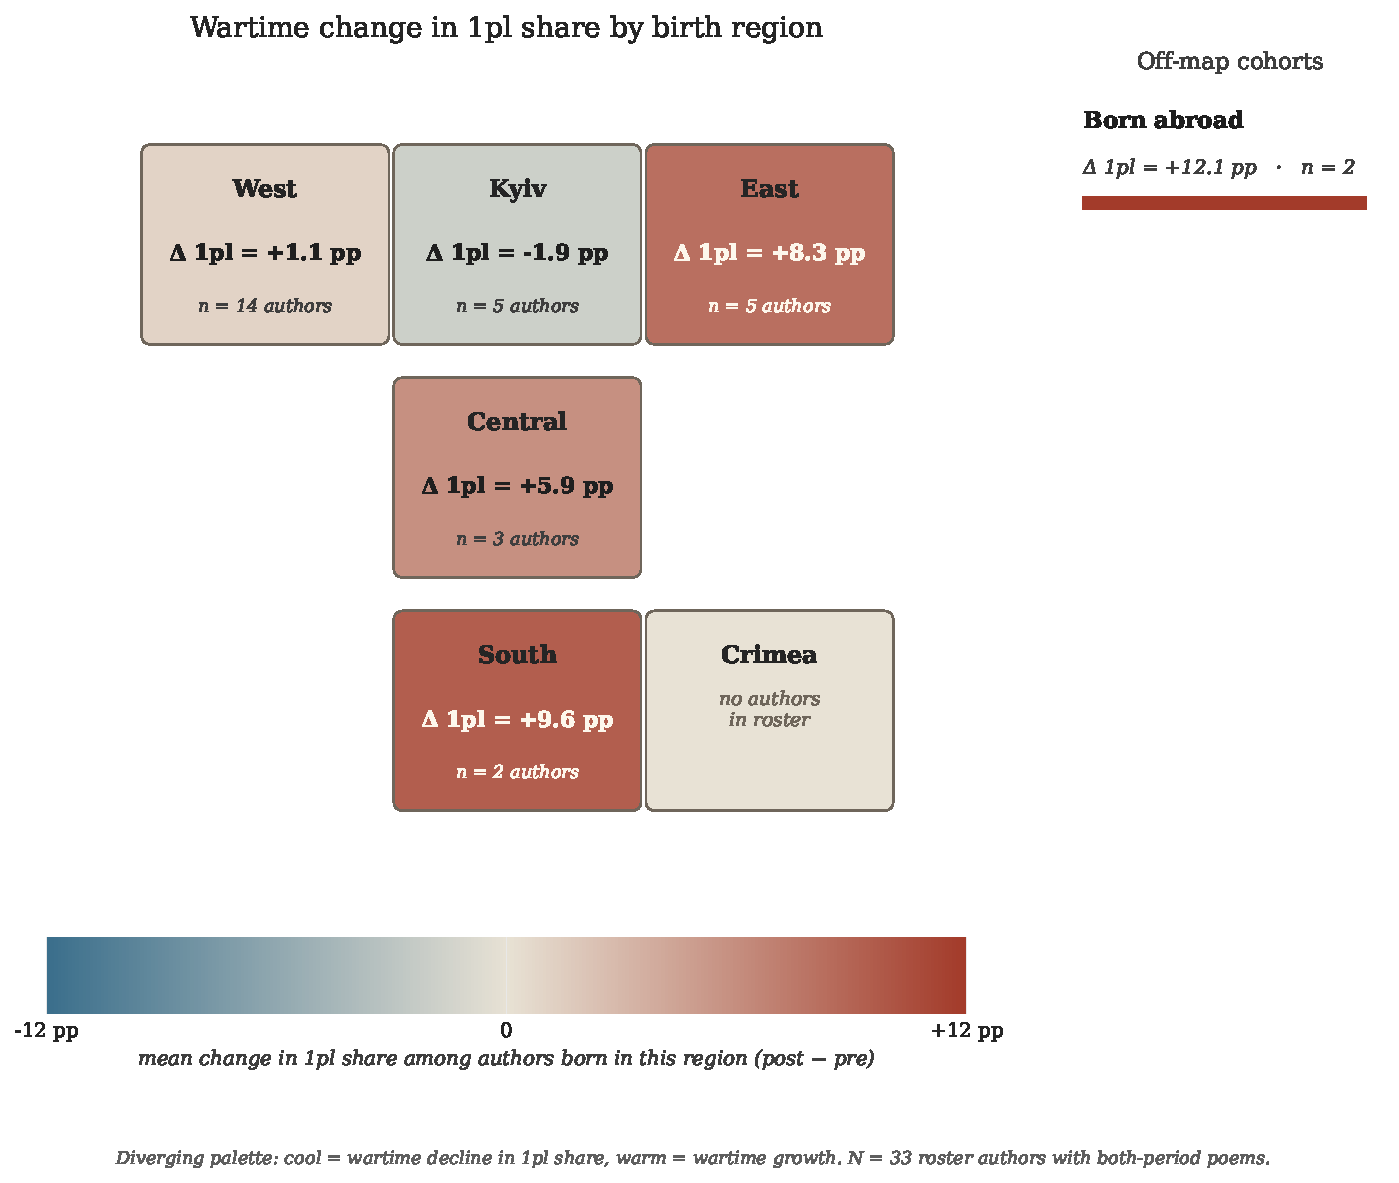
\includegraphics[width=0.95\textwidth]{fig_narr_3_ukraine_birthplace_map.pdf}
\caption{Stylized tile map of Ukrainian sub-regions colored by the mean post-2022 minus pre-2022 change in the 1pl share within the closed quartet, computed over roster authors born in that sub-region. Side panel: off-map cohorts (born abroad). Diverging colorscale: cool tones $=$ wartime decline in 1pl share; warm tones $=$ wartime growth. Author counts inset on each tile.}
\label{fig:disc-map}
\end{figure}

% \subsection{Methodological contribution}
% \label{sec:discussion-contribution}

% The findings above rest on a pipeline that joins three methodological pieces, none of which is by itself novel but whose combination addresses a problem that has limited computational pronoun analysis in pro-drop languages: how to count what isn't there, how to attribute the counts to identifiable speakers, and how to characterise what those counts refer to. Ukrainian and Russian, in common with most Slavic, Romance, and East-Asian languages, license null subjects whenever the referent is recoverable from verb morphology, and the missing subjects, in those languages, are systematically and overwhelmingly the first and second person, i.e.\ exactly the cells on which the present analysis turns. Surface tokenizers and rule-based morphological parsers cannot recover those omitted subjects; any count built on them undercounts 1P and 2P forms, and the undercount almost certainly varies by author, period, and register in ways that confound exactly the contrast of interest. We resolve this with a two-step LLM annotation that translates each stanza into Shakespearean English (whose obligatory explicit subjects and thou/ye singular--plural split provide a near-one-to-one mapping for the Ukrainian deictic inventory) before extracting pronoun counts from the translated surface form. The result is a pronoun inventory that recovers pro-dropped subjects rather than treating them as noise, and that preserves the 2sg/2pl contrast that English surface-form parsers collapse.

% The second piece is the within-author panel design. Treating each poet as their own control eliminates the between-author confounding that any cross-sectional analysis of literary corpora must otherwise contend with: differences in style, register, theme, training, language preference, and biographical context are absorbed into the author fixed effect (frequentist path) or the author random intercept (Bayesian path), and the period coefficient is identified from within-person change alone. The two-level architecture that pairs the per-cell frequentist GLM (RQ1) with the cell-by-author hierarchical NB (RQ2) is the empirical engine of the heterogeneous-reaction finding above: RQ1 establishes the corpus-level null under multiplicity control, RQ2 documents the structured author-level variance that the null integrates over, and the contrast between the two is what licenses the substantive claim that the invasion polarized rather than homogenized the deictic field.

% The third piece is the dependency-parsed collocation layer (RQ3). Where the rate-level analyses ask whether each pronoun cell shifts in frequency, the collocation layer asks which head verbs and nouns each pronoun cell governs, and tests those individual head lemmas under the same Benjamini--Hochberg multiplicity control \citep{benjamini1995controlling} that disciplines the cell-level inference. The pipeline adds nothing methodologically novel in isolation: dependency parsing of Slavic text is standard \citep{qi2020stanza}, and the log-likelihood ratio for collocation \citep{dunning1993accurate} together with BH-FDR control is the modern default in computational lexicography. Their joint use here, on a corpus whose pronouns are first recovered from pro-drop morphology via the Shakespearean-English layer and then dependency-parsed in Ukrainian and Russian directly, completes the architecture in a specific direction: the corpus-level RQ1 null is followed by an author-level RQ2 dispersion finding, which is in turn followed by an RQ3 lexical-syntactic localisation that names the verbs through which the dispersion operates.

% For Computational Social Science and Digital Humanities, the contribution of the combined pipeline is threefold. First, the LLM pro-drop pass demonstrates that morphologically rich pro-drop languages are no longer outside the reach of quantitative pronoun analysis: the same person--number contrasts that have grounded decades of English-language political-discourse work are now available, at scale, for Ukrainian and (with equivalent prompt engineering) for the larger Slavic-Romance-East-Asian space. Second, the within-author panel design ports econometric within-person identification into a literary corpus: each poet contributes their own pre/post contrast, the corpus aggregates those contrasts under multiplicity control, and the hierarchical layer recovers the heterogeneity that the aggregate suppresses, a workflow that translates with minimal adaptation to any longitudinal author-keyed corpus (legislative speeches, judicial opinions, autobiographical memoir, journalistic columns). Third, the three-level RQ1/RQ2/RQ3 architecture demonstrates that homogeneous-effect tests, heterogeneous-effect tests, and lexical-anchoring tests are complementary rather than competing: a corpus that reads as null on the mean can simultaneously document substantial structured heterogeneity at the individual level, and a localisable verbal restructuring at the collocate level, and the literary-studies and political-pragmatic readings of that heterogeneity (in the present case, the post-2022 polarization of the Ukrainian poetic ``we'') depend on having all three layers in evidence rather than choosing between them.

\section{Conclusions}

This study asked whether the full-scale invasion of 24 February 2022 left a detectable signature in the deictic grammar of contemporary Ukrainian and Russian-language poetry, and at what scale that signature is legible. Three converging analyses return a single, scale-dependent answer. At the corpus level (RQ1), no within-author person--number rate shift survives the confirmatory criterion of Poisson/negative-binomial agreement plus wild-cluster bootstrap survival of BH-FDR control, in either language stratum; the hierarchical Bayesian replication returns the same population-level null. At the author level (RQ2), that null dissolves into structured heterogeneity: random-slope dispersion on the open cells is comparable in magnitude to the population mean, and the 1pl cell in particular splits into a strongly positive cluster of poets with documented civic-military realignment and a negative cluster of older, Kyiv-resident, or displaced poets whose archives thin after 2022. At the lexical-syntactic level (RQ3), the collocation layer recovers a small set of multiplicity-controlled survivors that the rate models cannot see: the wartime Ukrainian 1pl acquires a deontic governor (\textukrainian{мусити}, ``must''), and the wartime Ukrainian 2sg an affective governor (\textukrainian{хотіти}, ``want''), each distributed across many poets, while the apparently dramatic Russian 1sg restructuring proves to be a pseudo-replication artifact of a single author once within-poem repetition is audited. The author-cluster decomposition localises the deontic ``we'' further still: it is carried by the non-frontline portion of the roster, whereas the frontline-mobilized poets articulate a 1pl whose governing verbs are existential rather than exhortational.

The substantive conclusion is therefore not that the invasion failed to move the poetic ``we,'' but that it did not move it homogeneously. The corpus mean is null because mobilization and retreat are averaged against one another; the invasion polarized the deictic field along biographical lines rather than crystallizing a single shared wartime collective. This reading is consistent with the Brubakerian account of groupness as a contingent, unevenly enacted event, with Onuch's generation-specific civic-identity thesis (the 1pl surge concentrates in the youngest fighting-age cohort), and with Reyes's legitimization framework (obligation grafted directly onto the in-group pronoun). Methodologically, the result also demonstrates that homogeneous-effect, heterogeneous-effect, and lexical-anchoring tests are complementary rather than competing: a corpus that reads as null on the mean can simultaneously carry substantial structured author-level variance and a localisable verbal restructuring, and the political-pragmatic interpretation depends on holding all three layers in evidence at once.

\section{Limitations}

Several limitations bound these conclusions. First, the roster is a small, self-selected literary sample drawn from a Facebook-circulated poetic field; it is not a probability sample of Ukrainian poetry, and the Russian-language stratum in particular ($14$ authors, with most post-2022 poems concentrated in a handful of writers) is too thin to support cell-level inference, as the non-robust Russian 2sg result and the Solomko-driven Russian 1sg cluster both illustrate. Second, the collocation layer rests on the Stanza universal-dependency pipeline, whose models were trained on prose; their accuracy on lyric stanzas with enjambment, inversion, and ellipsis is not formally validated here, so the dependency-relation and head-lemma attributions carry an unquantified parsing-error term. Third, the log-likelihood collocation test treats each pronoun--head co-occurrence as independent, an assumption that lyric anaphora violates through within-poem repetition; we mitigate this with a token-level pseudo-replication audit and report only distributionally robust survivors, but the audit is manual and cell-specific rather than a formal random-effects correction. Fourth, the pronoun inventory itself is reconstructed from pro-drop morphology by a two-step GPT-4o-mini annotation validated against only a $200$-stanza stratified human review; residual annotation error, particularly in the 2sg/2pl ({\ukrainianfont ти}/{\ukrainianfont ви}) contrast, propagates into every downstream estimate. Fifth, the author covariates are assembled from open biographical sources of uneven completeness: birthplace, post-2022 residence, and mobilization status are missing for some roster members (the Russian 1sg artifact author Solomko among them), which constrains the cluster and region-of-birth decompositions. Finally, the design is observational and the period contrast is not a controlled intervention: composition-year coding, archive-density changes, and shifting posting behavior across the cutpoint are partially confounded with the wartime contrast, so the period coefficients should be read as conditional associations within the modeled corpus rather than as causal effects of the invasion.

\section*{Acknowledgment}

An unnumbered section, e.g.\ \verb"\section*{Acknowledgements}", may be used for thanks, etc.\ if required and included \emph{in the non-anonymous version} before any Notes or References.


\section*{Disclosure statement}

An unnumbered section, e.g.\ \verb"\section*{Disclosure statement}", may be used to declare any potential conflict of interest and included \emph{in the non-anonymous version} before any Notes or References, after any Acknowledgments and before any Funding information.

\bibliographystyle{tfcad}
\bibliography{reference}

\appendix

\section{Roster sample composition}
\label{app:sample}

Figure~\ref{fig:app-sample} reports the cell-by-level frequencies of the four time-invariant author-level covariates used in the RQ2 random-slope model (gender, generation cohort, region of birth, and empirical period-1 language), restricted to the $33$ roster authors who enter the modeled sample. The figure documents the composition that the population-level posteriors in Table~\ref{tab:rq2-pop} integrate over and that the biographical clustering in \S\ref{sec:discussion-synthesis} reads against. The roster is gender-balanced ($13$ female, $20$ male), generationally concentrated in the 1980s cohort ($n = 14$) and the pre-1970 cohort ($n = 9$), regionally over-weighted to West-Ukraine ($n = 14$) and Kyiv / East-Ukraine ($n = 5$ each), and linguistically dominated by Ukrainian-primary writers ($n = 27$) over Russian-primary writers ($n = 6$).

\begin{figure}[h]
\centering
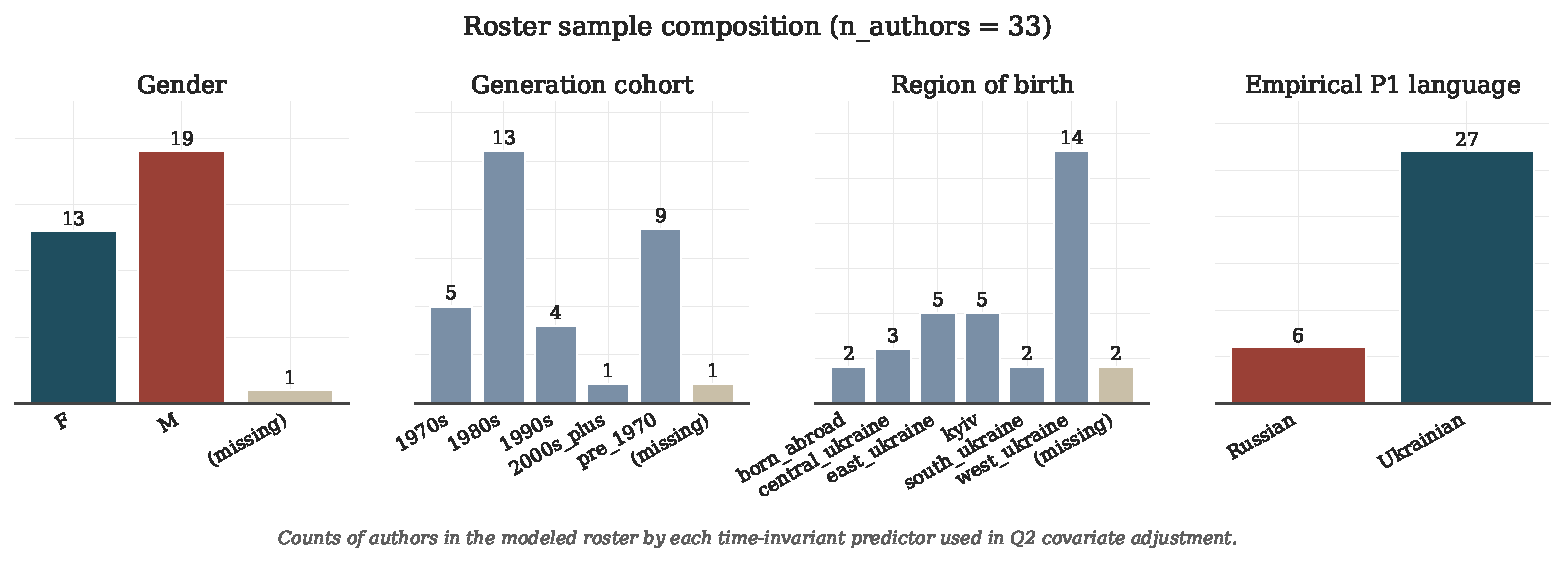
\includegraphics[width=0.98\textwidth]{fig_narr_6_roster_sample_composition.pdf}
\caption{Counts of authors in the modeled roster by each time-invariant covariate used in the RQ2 covariate-adjusted sensitivity layer ($n_{\text{authors}} = 33$). The four panels (gender, generation cohort, region of birth, empirical period-1 language) are the same factors that enter the hierarchical model in \S\ref{sec:results-rq2} and that anchor the biographical interpretation in \S\ref{sec:discussion-synthesis}.}
\label{fig:app-sample}
\end{figure}

\section{Author trajectories}
\label{app:trajectories}

\begin{figure}[h]
\centering
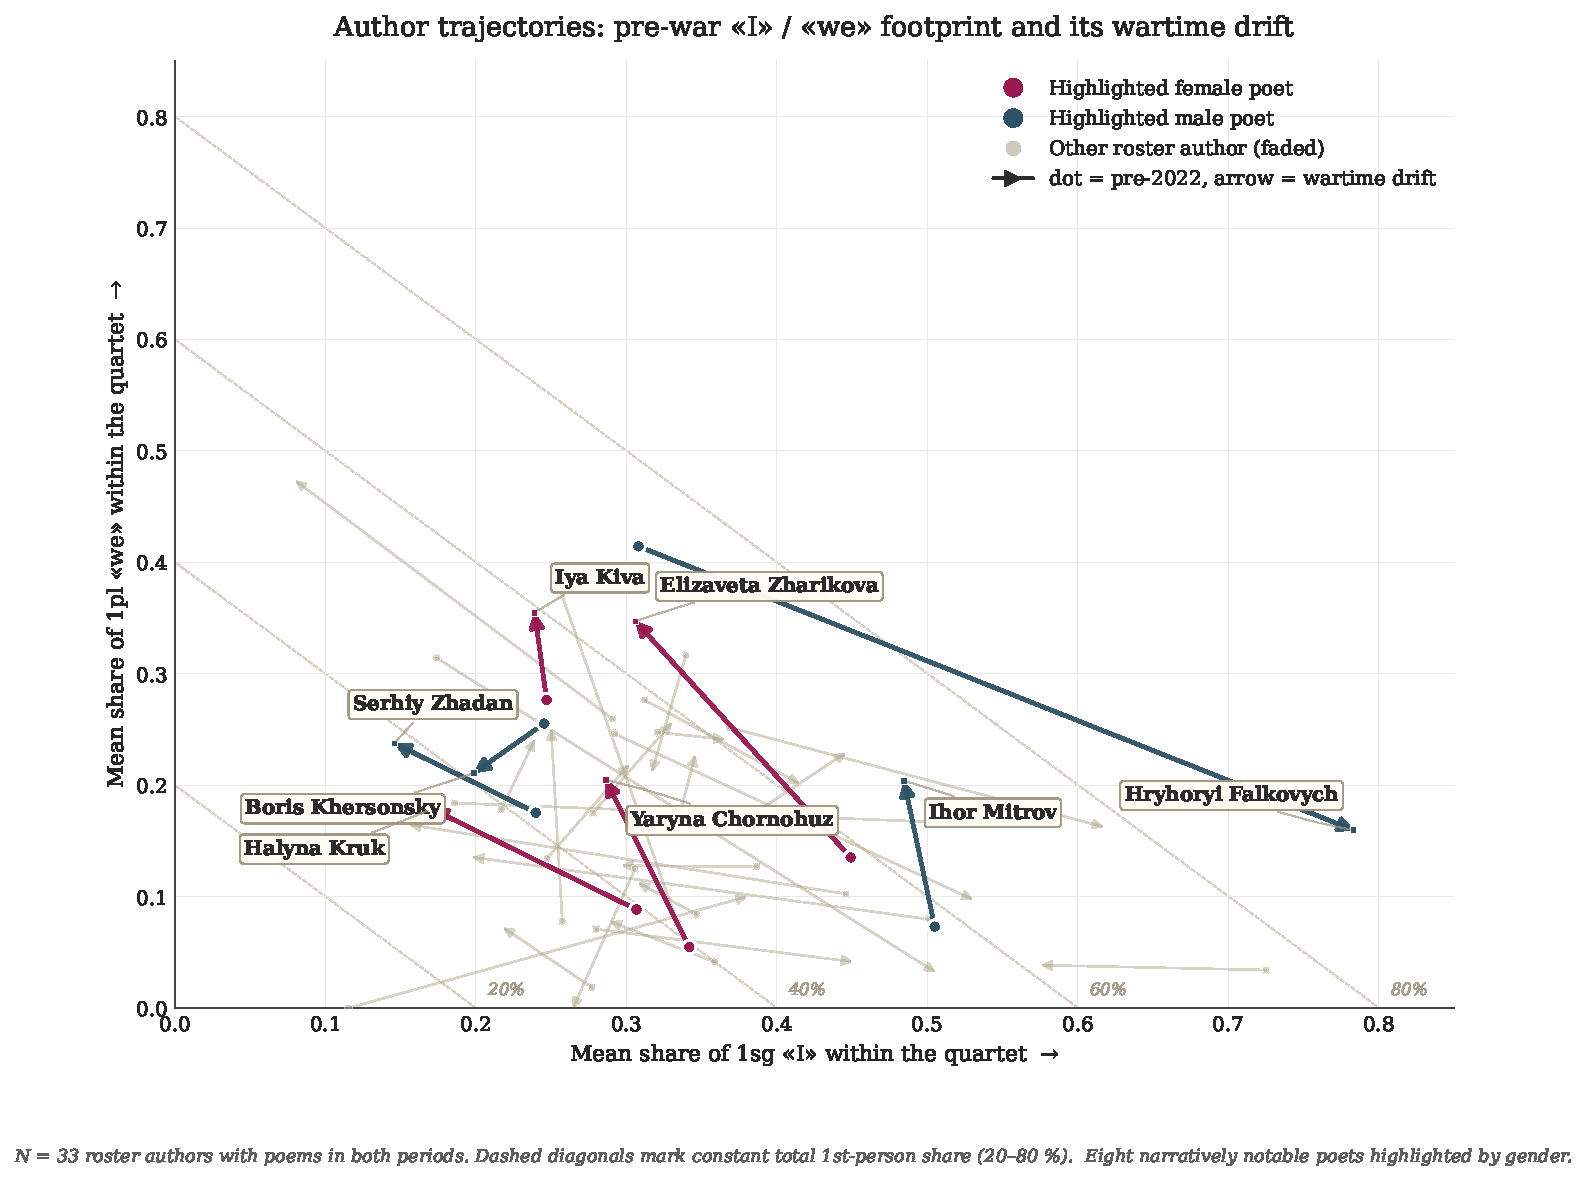
\includegraphics[width=0.98\textwidth]{fig_narr_2_author_trajectories.pdf}
\caption{Author trajectories in the (1sg-share, 1pl-share) plane of the closed first/second-person quartet. Each arrow runs from the author's pre-2022 mean position (dot) to their wartime position (arrowhead). Faded cream arrows: full roster ($n = 33$). Highlighted colored arrows: eight narratively notable authors keyed by documented wartime situation---crimson: mobilized (frontline / civic-military); deep teal: residentially stable; bronze: displaced (in-country or abroad). Colour encodes biographical situation; the arrow direction carries each poet's 1pl drift. Dashed grey diagonals mark constant total-1st-person share isolines.}
\label{fig:rq2-trajectories}
\end{figure}

\section{Breakpoint regression and PELT change-point detection}
\label{app:breakpoint}

\begin{figure}[h]
\centering
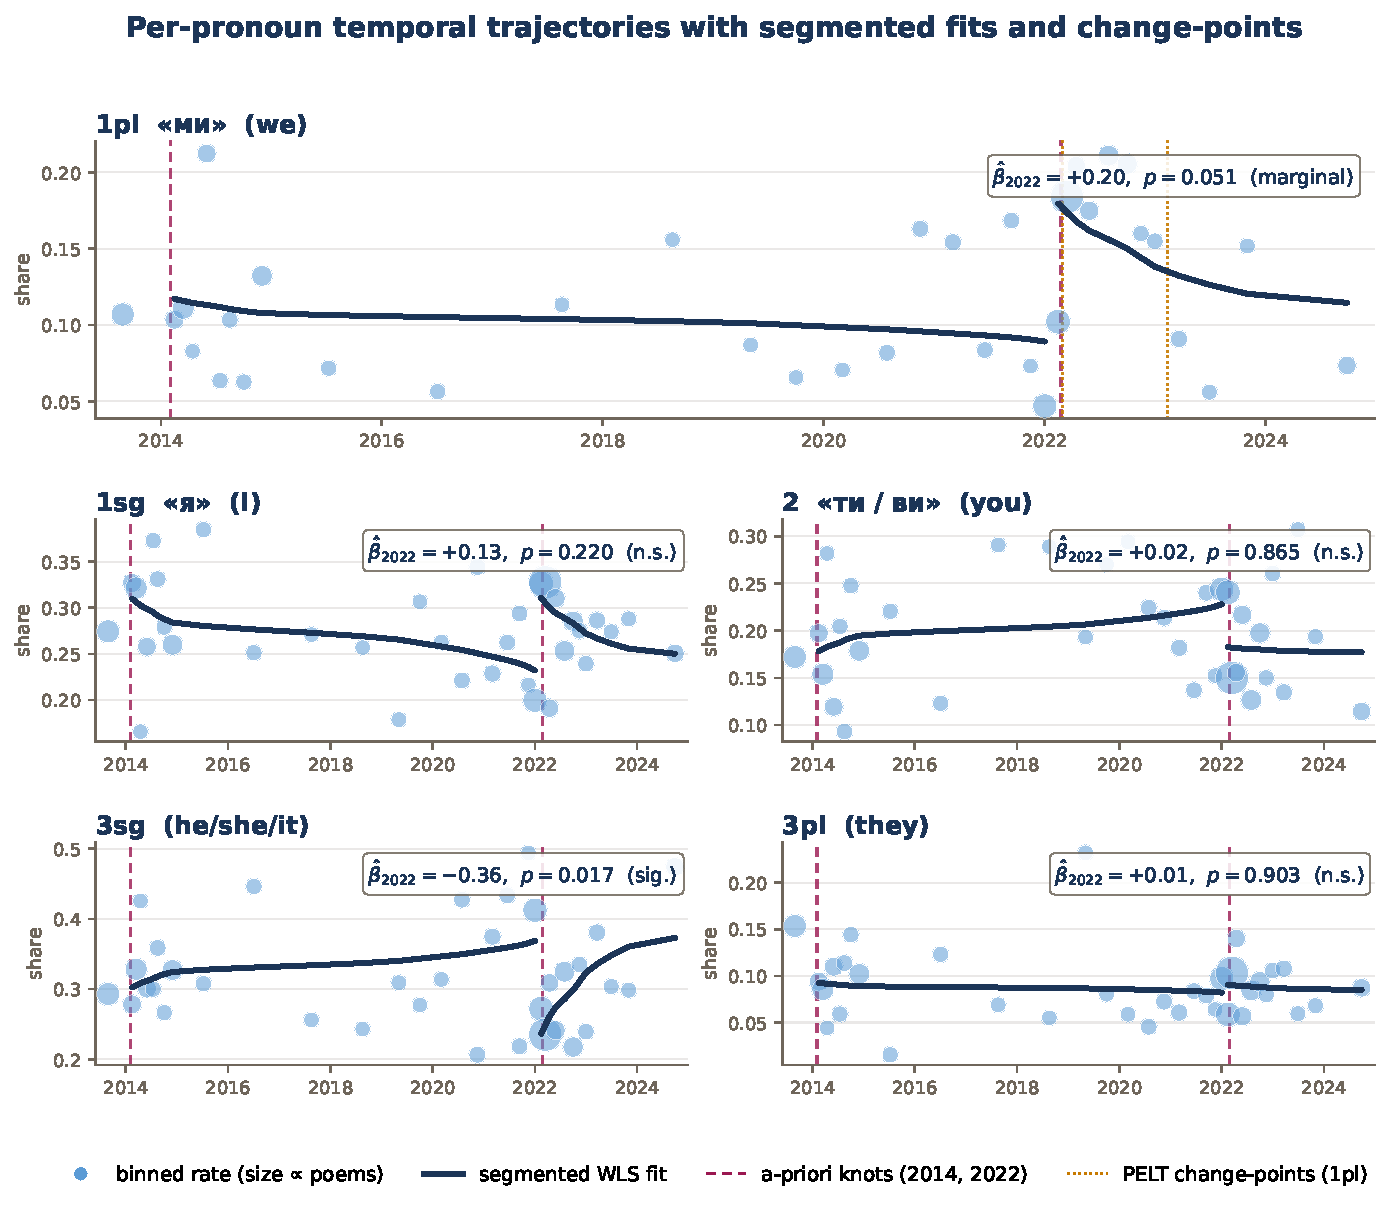
\includegraphics[width=\textwidth]{fig1_breakpoint_timeseries.pdf}
\caption{Adaptive temporal binning (35 bins, each with $\geq 30$ poems) of per-stanza pronoun rates over 2013--2025 on a calendar-time axis. Each point is a bin (size $\propto$ poem count); the dark line is the segmented weighted-least-squares fit, drawn as explicit level steps at the two a-priori knots (2014, 2022). The enlarged top panel is the headline 1pl series, which exhibits a marginal level shift at the 2022 knot ($\hat{\beta}_{2022} = +0.20$, $p = 0.051$) and two PELT change-points (2022-03-01, 2023-02-10) bracketing the invasion; remaining cells follow in the lower grid. 1sg shows a confirmed 2014 level shift but is stable across 2022; 3sg drops sharply at 2022 ($\hat{\beta}_{2022} = -0.36$, $p = 0.017$); the 2 (\textukrainian{ти}/\textukrainian{ви}) and 3pl trajectories are null at both knots.}
\label{fig:rq1-breakpoint}
\end{figure}

\end{document}
